\chapter{Virtualization Overhead}


Operating systems typically provide a basic set of resource virtualization facilities. These facilities enable the operating system to share physical resources among the applications through the implementation of virtual memory, CPU schedulers, and process hierarchies. However, these facilities are not sufficient in a context where some applications require operating environments that differ from the needs of other applications running on the same machine. As discussed in chapter 3, several virtualization solutions address the resource isolation needs by virtualizing key system resources (CPUs, memory, disks, network interfaces). To transparently abstract system resources, most virtualization solutions perform redundant operating system functions, including CPU scheduling, memory management, network stack implementation, and disk I/O. For example, an application running on a virtual machine is scheduled on the virtual CPUs (VCPUs) by the guest operating system, while the VCPUs are in turn scheduled on the physical CPUs by the host operating system. This redundancy imposes overhead on the use of system resources. The virtualization overhead varies based on the implementation of the virtualization system. A key goal of any virtualization technique is to impose as little overhead as possible, while providing the needed resource isolation. 

This chapter evaluates the representative virtualization solutions introduced in Chapter 3 based on the virtualization overhead they impose under varying operating conditions and workloads. First, we evaluate the solutions based on the overhead they impose in virtualizing access to CPUs. Second, we measure the overhead associated with memory access bandwidth available to applications running within a virtual machine. Third, we study the impact of virtualization on network access bandwidth. Fourth, we measure the overhead associated with disk I/O operations, focusing on sequential and random file access operations, and general disk access latency. Fifth, we measure the performance of each of the virtualization platforms using the standard system benchmarks. Finally, we measure the performance of the Intelligent River\textsuperscript{\textregistered} middleware components under each of the virtualization platforms.


\section{Experimental Conditions}

To evaluate the three representative virtualization solutions independently, and to be able to compare the results with the performance on an independent bare-metal host, we used four identical Dell Optiplex 990 machines with the following configuration:
\newline
\begin{table}[h!]
\begin{center}
\renewcommand{\arraystretch}{1.5}
\begin{tabular}{ | l | l | }
  \hline                        
  Processor & Intel(R) Core(TM) i7-2600 CPU @ 3.40GHz \\ \hline
  Chipset & Intel(R) Q67 Express Chipset \\ \hline
  Memory & 8 GB, Non-ECC Dual-Channel 1333 MHz DDR3  \\ \hline
  Network & Intel (R) 82579LM Ethernet LAN 10/100/1000 \\ \hline
  Hard disk & 1TB 7200 RPM SATA 3.0Gb/s \\
  \hline  
\end{tabular}
\end{center}
\caption{Experimental Setup - Hardware Configuration}
\end{table}


To ensure a fair comparison, we preserve the default operating system and hypervisor configurations. Modification of any default settings required to evaluate specific scenarios noted. The default operating system, kernel, and hypervisor settings are as follows:
\newline

\begin{table}[h!]
\begin{center}
\renewcommand{\arraystretch}{1.5}
\begin{tabular}{ | l | l | }
  \hline                        
  Operating system & Ubuntu Server 12.04.3 LTS \\ \hline
  Kernel & GNU/Linux 3.8.0-29-generic x86\textunderscore 64 \\ \hline
  Lxc version & 0.7.5  \\ \hline  
  QEMU-KVM version & 1.0  \\  \hline 
  Xen version & xen-3.0-x86\textunderscore 64 hvm-3.0-x86\textunderscore 64  \\ \hline
\end{tabular}
\end{center}
\caption{Experimental Setup - Software Configuration}
\end{table}

\newpage
\section{CPU Overhead}

Most virtualization solutions rely on the creation of virtual CPUs, with the hypervisor responsible for scheduling the virtual CPUs over the physical CPUs. This creates an additional layer of control, which makes it possible to create  virtual CPUs that are in turn backed by more than one physical CPU. Alternatively, virtualization also enables creation of more virtual CPUs than physical CPUs available on the system. The CPU capacity available to the applications in a virtualized environment is influenced by two parameters, (i) the raw performance of the CPU in executing primitive tasks, and (ii) the performance of the scheduler in scheduling multiple threads.


To evaluate CPU overhead, we created a sample application (w1) representing a diverse set of CPU-oriented tasks:
\begin{enumerate}
 \item Repeated calculation of large prime numbers using varying numbers of threads.
 \item Measuring the speed and efficiency of floating point operations including sin, cos, sqrt, exp, log, array accesses, conditional branches, and procedure calls by executing the whetstone workload from the unixbench suite of tests \cite{unixbench}.
 \item Execution of a large number of threads competing for a set of mutexes, in order to measure the scheduler performance for multi-threaded applications \cite{sysbench}.
 \item Generation of 500 RSA private keys using openssl \cite{openssl}.
 \end{enumerate}  

The objective of this test suite is to measure the execution time of the sample application and its individual tasks as described above. The tests were performed on a virtual machine created on each of the three virtualized servers, and also on an independent bare-metal system used as a baseline.

\begin{figure}[H]
\centering
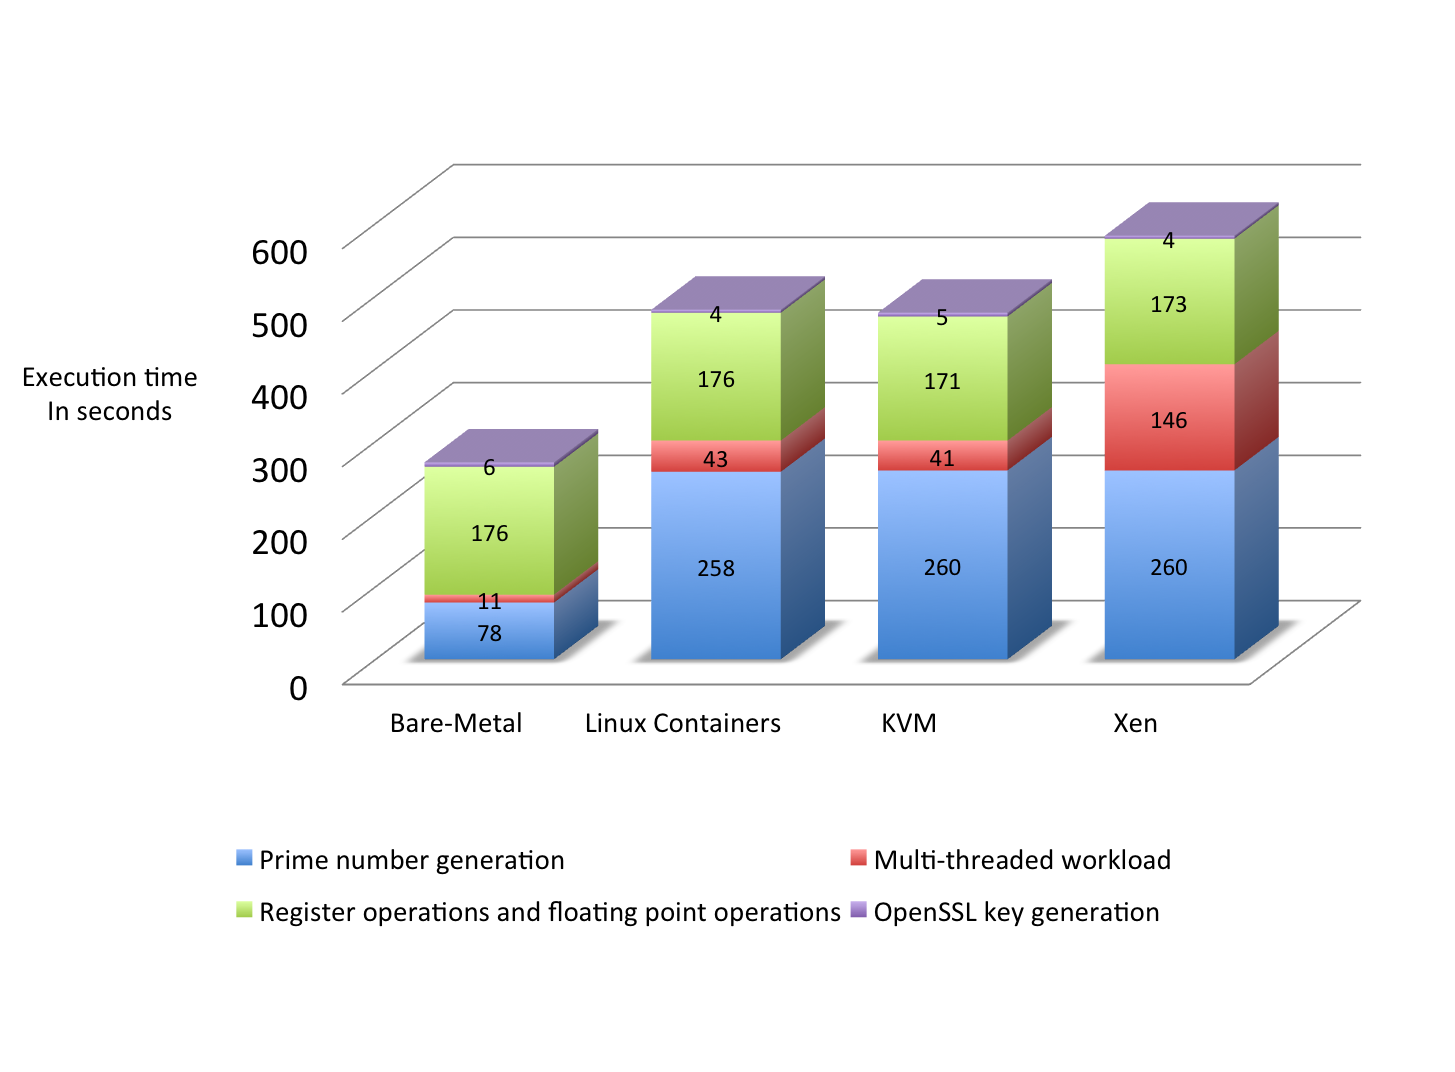
\includegraphics[width=140mm]{1cpu.png}
\caption{CPU Virtualization Overhead - 1 Virtual CPU}
\label{fig:1cpu}
\end{figure}

A virtual machine was created on each of the three physical servers, each with one virtual CPU, 300 GB of disk storage and 7680 MB of memory. Figure \ref{fig:1cpu} shows the overhead introduced by the representative virtualization platforms while virtualizing a single VCPU over one of the eight physical CPUs. The X-axis represents the virtualization platform, and the Y-axis represents the (stacked) execution time of the sample application (w1). It is evident from Figure \ref{fig:1cpu} that virtual machines created using Linux containers and KVM executed the sample application faster than the virtual machine created using Xen. Xen, among the three virtulization solutions, yielded higher overhead with respect to CPU access. In particular, Xen took longer to complete the task involving multiple threads competing for a set of mutexes, indicating the poor relative performance of the CPU scheduler in the Xen hypervisor.


\begin{figure}[H]
\centering
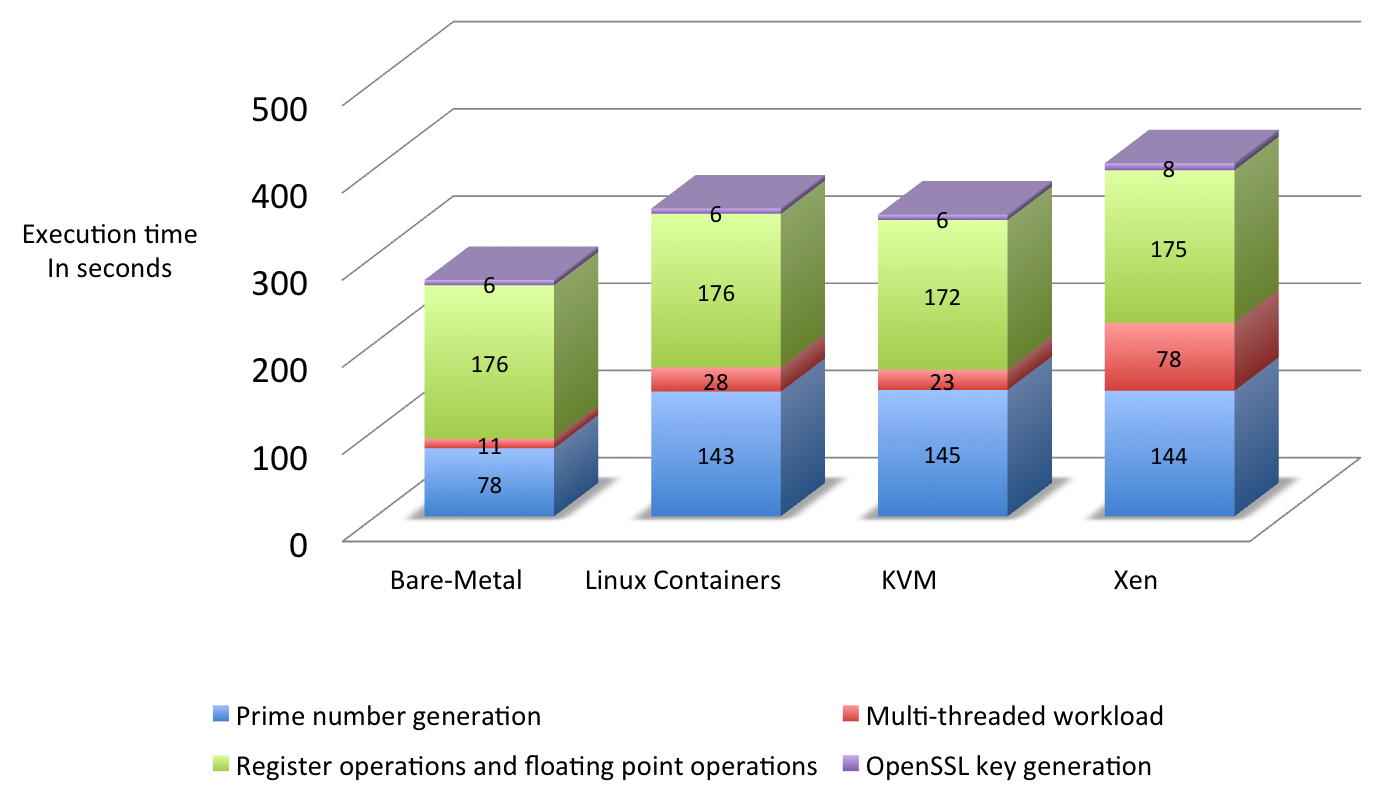
\includegraphics[width=140mm]{2cpu.png}
\caption{CPU Virtualization Overhead - 2 Virtual CPUs}
\label{fig:2cpu}
\end{figure}

The same test was repeated with the virtual machines configured with two virtual CPUs mapped to two of the physical CPUs, 300 GB of disk storage, and 7680 MB of memory. The execution times with the modified configuration are shown in Figure \ref{fig:2cpu}. The single threaded tasks were not affected by the availability of an additional core and were executed in almost the same time as the previous test. Note that the execution times for the multi-threaded tasks are lower compared to the results in Figure \ref{fig:1cpu}, owing to the availability of one additional physical core. The results once again bring out the poor scheduler performance of the Xen hypervisor.

\begin{figure}[h]
\centering
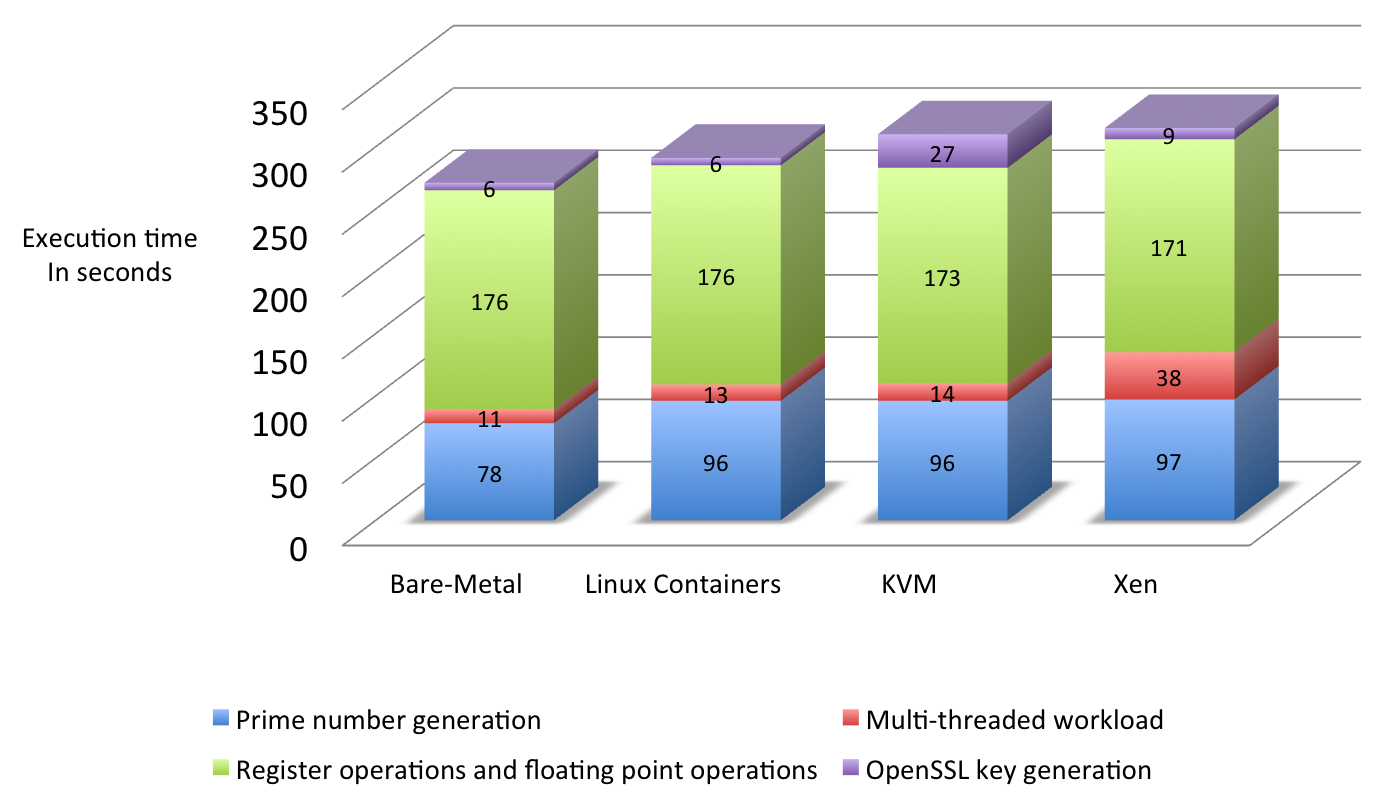
\includegraphics[width=130mm]{4cpu.png}
\caption{CPU Virtualization Overhead - 4 Virtual CPUs}
\label{fig:4cpu}
\end{figure}


The same test was repeated with the virtual machines configured with four virtual CPUs mapped to four of the physical CPUs, 300 GB of disk storage, and 7680 MB of memory. The execution times with the modified configuration are shown in Figure \ref{fig:4cpu}. The results once again confirm our hypothesis from the previous tests about the poor performance of the Xen scheduler for multi-threaded workloads.

\begin{figure}[H]
\centering
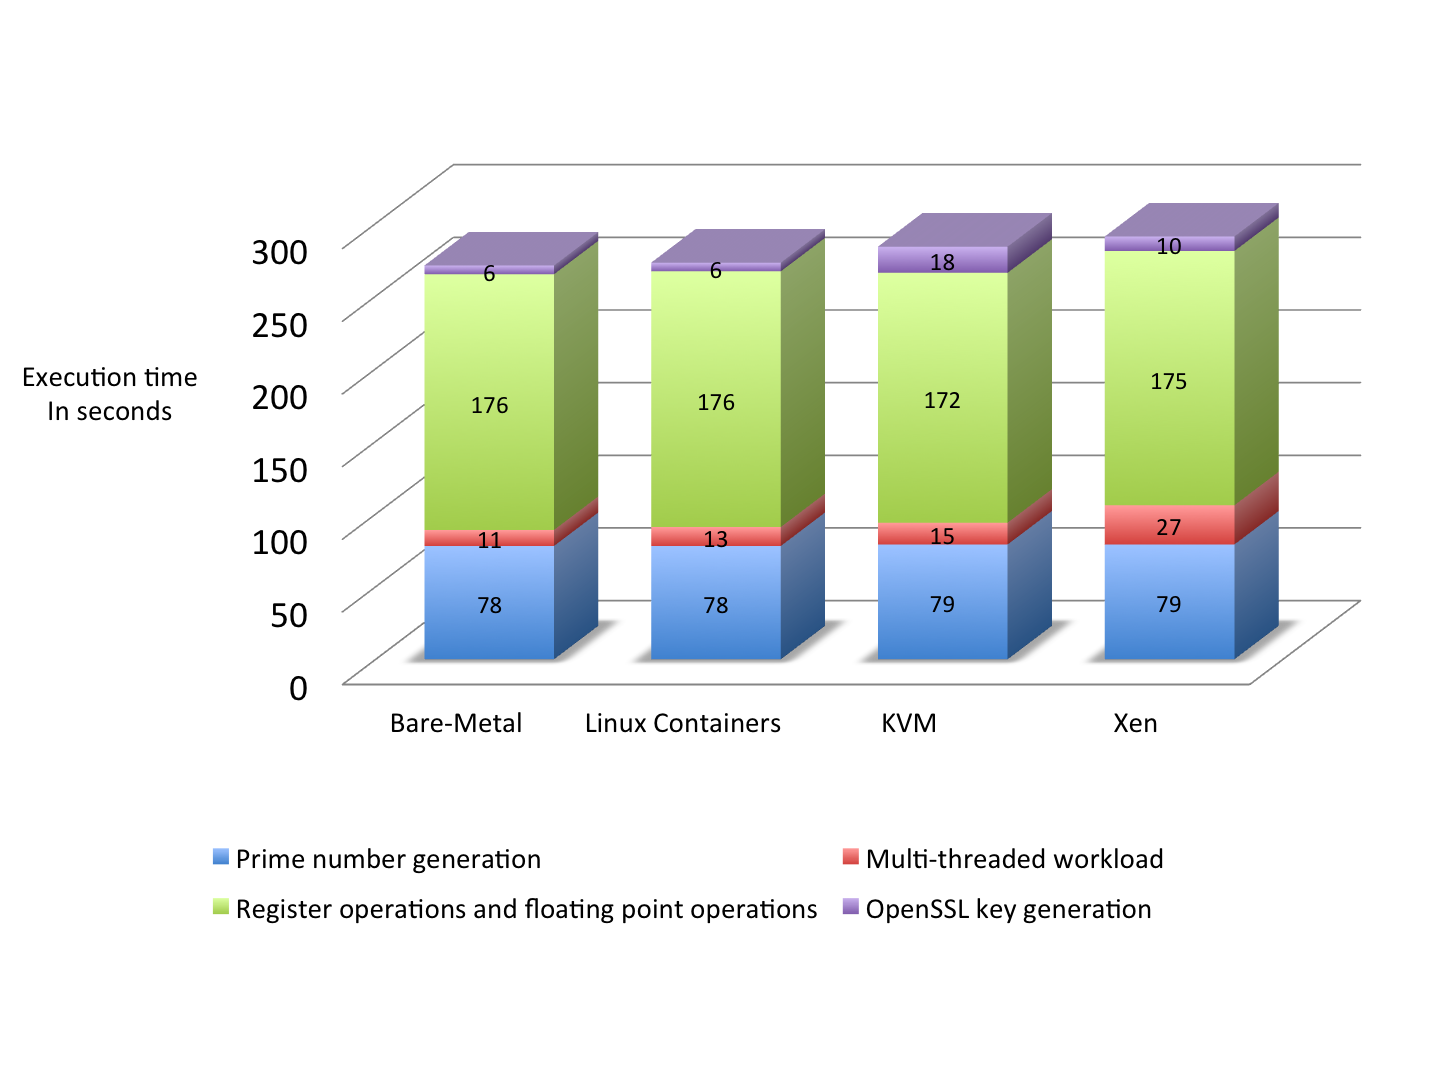
\includegraphics[width=130mm]{8cpu.png}
\caption{CPU Virtualization Overhead - 8 Virtual CPUs}
\label{fig:8cpu}
\end{figure}

To further examine the overhead introduced when virtualizing the CPUs, we ran the test again, with the virtual machines configured eight virtual CPUs mapped to eight physical CPUs, 300 GB of disk storage, and 7680 MB of memory. The resources available to the virtual machines were identical to the bare-metal host, with the only exception being an added hypervisor. The difference in execution times among the virtual machines representing Linux containers, KVM, and Xen and the bare-metal host can be correlated with overall CPU overhead. Both Linux Containers, and KVM exhibit the least overhead, followed by Xen.

Based on these results, we conclude that Linux Containers and KVM perform the best for both single-threaded and multi-threaded workloads, exhibiting the least overhead compared to the bare-metal performance. Though Xen performed identically to the others for single-threaded workloads, it exhibited relatively poor performance when scheduling multi-threaded workloads.  

\section{Memory Overhead}

KVM, Xen, and Linux Containers manage virtual machine memory differently. Xen, being a para-virtualized platform, manages  virtual machine memory in a collaborative fashion. The Xen hypervisor allocates the required memory on the host, holds a section of the virtual machine's address space, and then decouples the virtual machine for any unprivileged memory accesses. Any sensitive instructions originating from the virtual machines are directed to the hypervisor. The virtual machines manage their own page tables. KVM, as a full virtualization solution, allocates the required memory on the host, and then decouples its virtual machines, allowing each to manage its own memory. The KVM kernel module provides each virtual machine its own address space in the host kernel. The memory allocated for each virtual machine is allocated in the virtual memory of the host. This design creates an interesting possibility where virtual machines can be created with total memory that exceeds the physical memory of the host. If a virtual machine attempts to use more memory than the host can provide, the host kernel starts its swapping process. The virtual machines are responsible for their own page tables. Linux containers, as an operating system virtualization solution, rely on the simplest memory management mechanism. Since containers share the kernel with the host, they do not maintain a separate page table. The containers are represented as a group of processes in the host kernel. Hence, the memory associated with the containers is just the virtual memory allocated for the corresponding process groups in the kernel.


To evaluate the virtualization overhead associated with memory access, we created a sample application (w2) that uses mbw \cite{mbw} to allocate two arrays of a given size, and then copies data from one to the other. The reported ``bandwidth'' is the amount of data copied, over the time required for the operation to complete. The objective of this test is to measure the memory access bandwidth available to the virtual machine created on each of the three virtualized servers, compared to the bandwidth observed on an independent bare-metal host.

\begin{figure}[H]
\centering
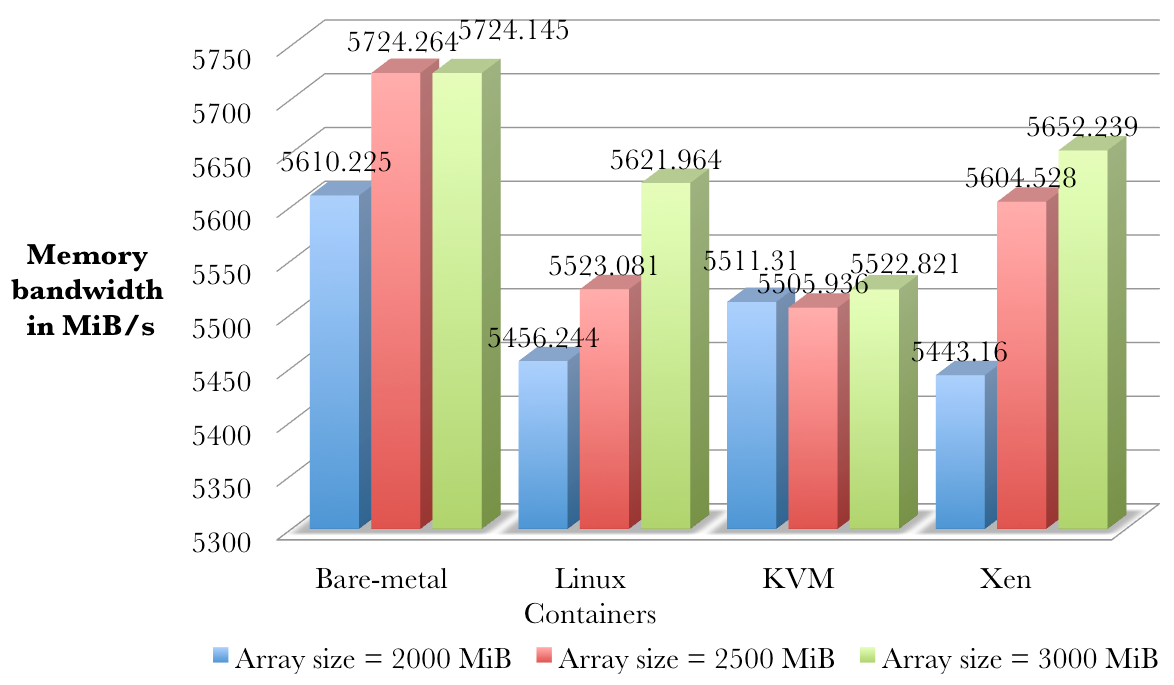
\includegraphics[width=130mm]{mem1.png}
\caption{Memory Virt. Overhead - (Virtual Machine Memory = Host Memory = 8 GB)}
\label{fig:mem1}
\end{figure}

A virtual machine was created on each of the three physical servers with eight virtual CPUs mapped to eight physical CPUs, 300 GB of disk storage, and 7680 MB of memory. In this case, since the virtual machine memory is equal to the host memory, the difference in memory access bandwidth between the virtual machines and the bare-metal host corresponds to the memory overhead caused by the virtualization platforms. The results are shown in Figure \ref{fig:mem1}, with the X-axis representing the virtualization platforms, and the Y-axis representing the observed bandwidth in mebibyte per second (MiB/s) for different array sizes. It is evident from the results shown in Figure \ref{fig:mem1} that each of the virtualization platforms exhibits a different overhead pattern. First, Xen exhibits high overhead for smaller array sizes indicating a less than average performance in the normal scenario. However, Xen performs relatively better for larger array sizes. This behavior is explained by the decoupling of memory management to the virtual machines themselves by the Xen Hypervisor. However, KVM showed an average memory overhead irrespective of the array size. This behavior is explained by the isolation of virtual machine memory in its own guest address space in the host and managing a mapping between the host address space and the guest address space. While the host is managing the memory allocated to a KVM guest, the guest kernel is simultaneously managing the same memory. To make optimal memory decisions and re-use identical pages among the virtual machines, the host kernel and the guest kernel collaborates using a feature called ``Kernel Same page Merging'' \cite{ksm} causing an overhead in low utilization scenarios.

\begin{figure}[H]
\centering
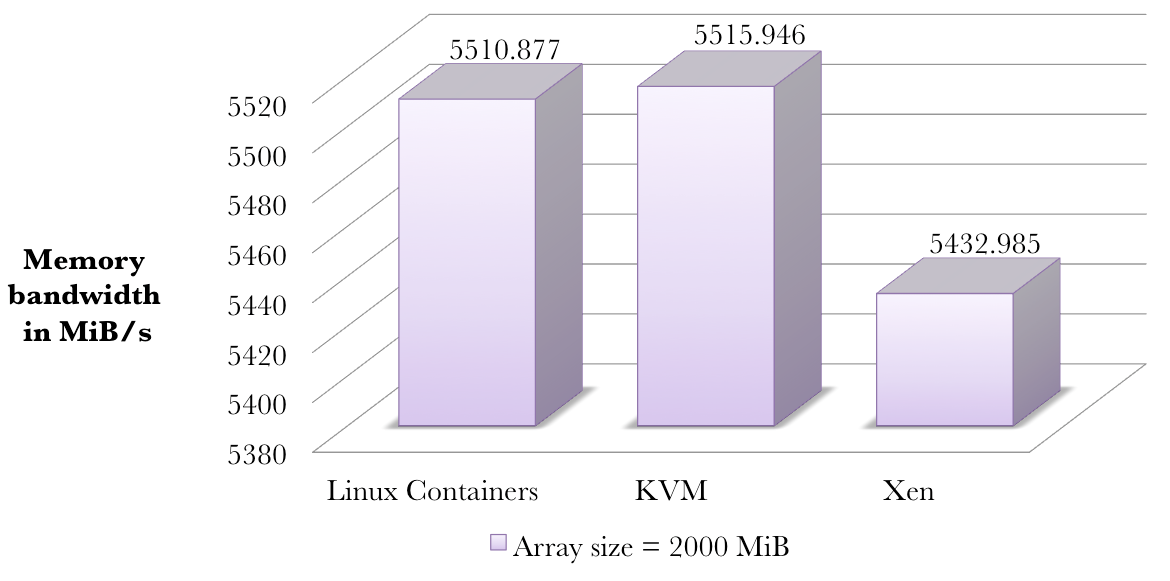
\includegraphics[width=130mm]{mem2.png}
\caption{Memory Virt. Overhead (Virtual Machine Memory(5 GB) \textless  Host Memory(8 GB))}
\label{fig:mem2}
\end{figure}


To further examine the behavior of the virtualization platforms when all of virtual machine memory can be accommodated by the host, we repeated the same test with the virtual machines configured with 5 GB of memory, 8 virtual CPUs mapped to 8 physical CPUs, and 300 GB of disk storage. As evident from the results shown in Figure \ref{fig:mem2}, Linux Containers and KVM yielded higher memory bandwidth than Xen.

\begin{figure}[H]
\centering
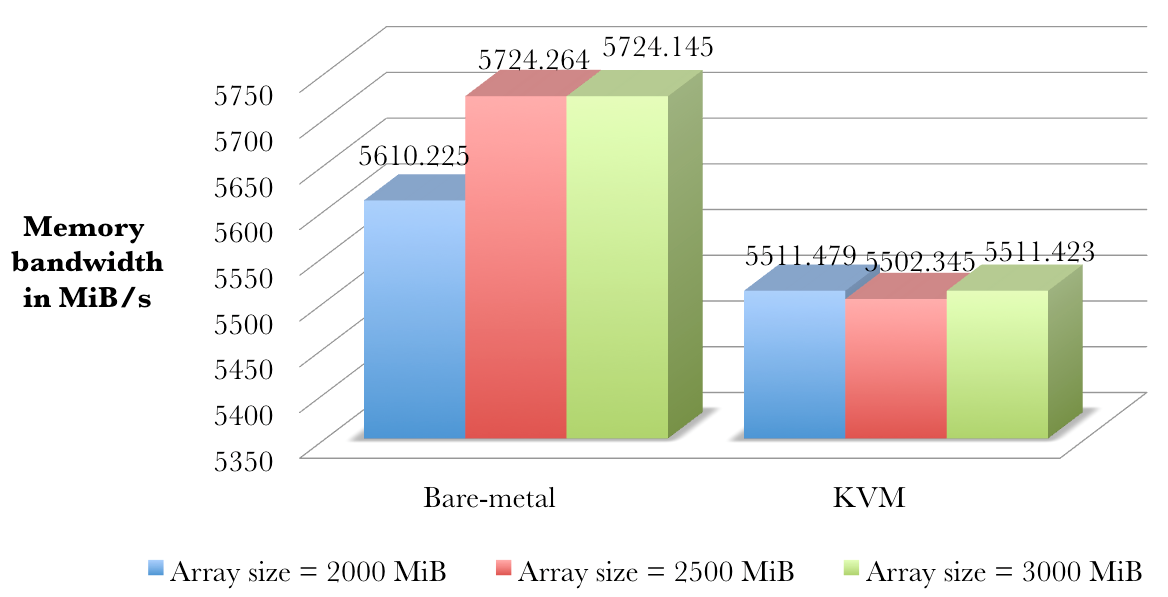
\includegraphics[width=130mm]{mem3.png}
\caption{Memory Virt. Overhead - Virtual Machine Memory(10 GB) \textgreater  Host Memory(10 GB)}
\label{fig:mem3}
\end{figure}

KVM allows virtual machines to run their own kernel, yet manages the virtual machine memory from the host kernel. As a result, it provides the ability to leverage memory over commitment facilities. Memory pages requested by a virtual machine are not allocated until they are actually used. The host kernel can free up memory by swapping less frequently used pages to disk. While not perfect, these techniques can be used to create extremely over-committed environments. To evaluate the behavior of KVM in such an over-committed environment, we created a virtual machine with 10 GB of memory virtualized on 8 GB of host memory, and observed the memory access bandwidth. The results, shown in Figure \ref{fig:mem3}, confirm our claim that KVM performs the same, even in an over-committed environment $-$ until all virtual machines attempt to use their share of memory at the same time. 


\section{Network Overhead}

KVM, Xen, and Linux Containers provide mechanisms to transparently virtualize network interfaces on the host, enabling the hosted virtual machines to build independent network stacks over their virtual network interfaces. KVM uses QEMU to emulate virtual network devices over the physical network interfaces. Xen enables virtual machines to use para-virtual drivers to access the network interfaces on the host. Linux Containers use network namespaces to virtualize container network interfaces. The virtual machines use their virtual networking facilities to communicate with external networks, as well as other virtual machines running on the same host. The network access available to a virtual machine can be : (i) network address translated (NAT), where the host proxies communications from the virtual machine, or  (ii) bridged, where the virtual machine is allowed to participate in the same LAN segment as the host. To measure the overhead associated with virtualizing networking interfaces, we measured the network bandwidth available to a virtual machine in both NAT and bridged configurations and compared the results with the bandwidth available on an independent bare-metal host. To ensure fair comparison, we set up an Iperf \cite{iperf} server on a machine outside the test network and measured the network bandwidth by running an iperf client on each of the virtual machines. The results are shown in Figure \ref{fig:net1}, where the X-axis represents the virtualization platforms, and the Y-axis represents the observerved network bandwidth in MBytes/sec.

\begin{figure}[H]
\centering
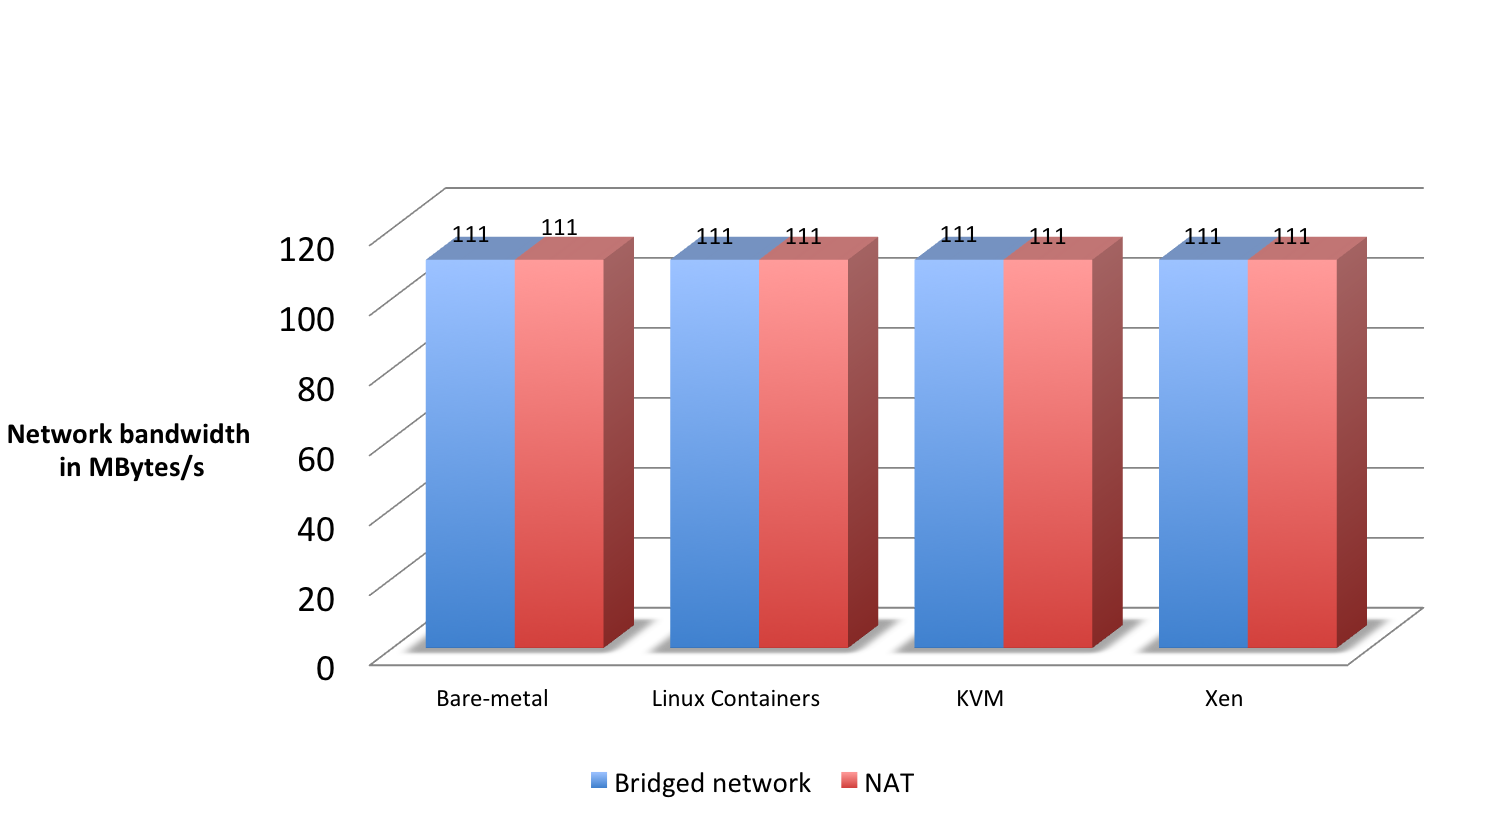
\includegraphics[width=130mm]{net1.png}
\caption{Network Virtualization Overhead - Network Bandwidth}
\label{fig:net1}
\end{figure}

It is evident from the results that there is no observable overhead introduced when virtualizing network interfaces using KVM, Xen, and Linux Containers.


\section{Disk I/O Overhead}

KVM, Xen, and Linux Containers handle disk I/O differently. Xen, being a para-virtualized platform, performs disk I/O with the help of para-virtual drivers. Xen does not expose the disk devices to the virtual machines. When the system boots, dom0 (the privileged domain) sets up the driver domains, which then serve as the hardware interfaces for all virtual machines that require disk access. Communication between the virtual machines and the driver domains occurs in memory. The software layer between the virtual machines and the physical layer driver leaves room for interesting optimization strategies in terms of shared memory, virtual interrupts, and grant tables, thereby reducing disk I/O overhead. 

KVM, as a full-virtualization platform, uses QEMU to create virtual devices that map to physical hardware. This mapping introduces additional overhead, as disk access is dependent on QEMU, which is single-threaded, presenting scalability limitations. The ``Big QEMU lock'' is an expensive mechanism in the path to the disk \cite{bql}. More recently, development efforts have shifted to para-virtual drivers for KVM. Currently, KVM supports two para-virtual drivers, virtio-blk \cite{virtioblk} and virtio-scsi \cite{virtioscsi}. Virtio drivers could also be used to access file-backed storage. For example, a virtual machine can access a file on the host operating system as a virtual disk using the virtio drivers. At the time of writing, development efforts are focused on ``virtio-blk-data-plane'', which provides an accelerated data path for para-virtual drivers using dedicated threads and Linux Aio \cite{aio} entirely bypassing the QEMU block driver \cite{blkdataplane}. The system under evaluation for this thesis runs the stable version of QEMU and uses virtio drivers to access a file-backed virtual disk.  

Linux Containers take the simplest route to implement disk I/O. A container's storage is represented as another directory on the host file system. Hence, each container uses the host's file system in an isolated fashion. The containers under evaluation for this thesis utilize a separate logical volume on the host to create its root file system.


To evaluate the overhead introduced when virtualizing disk I/O, we created a sample application (w4) that uses sysbench\cite{sysbench}, ioping \cite{ioping}, and dd \cite{dd} to perform sequential and random disk I/O. The objective of this test is to observe the execution time of the sample application and its individual tasks. The tests were performed on virtual machines created on each of the three virtualized servers, as well as an independent bare-metal system used as a baseline. The virtual machine was configured with 8 virtual CPUs mapped to 8 physical CPUs, 300 GB of disk storage, and 7680 MB of memory.

\begin{figure}[H]
\centering
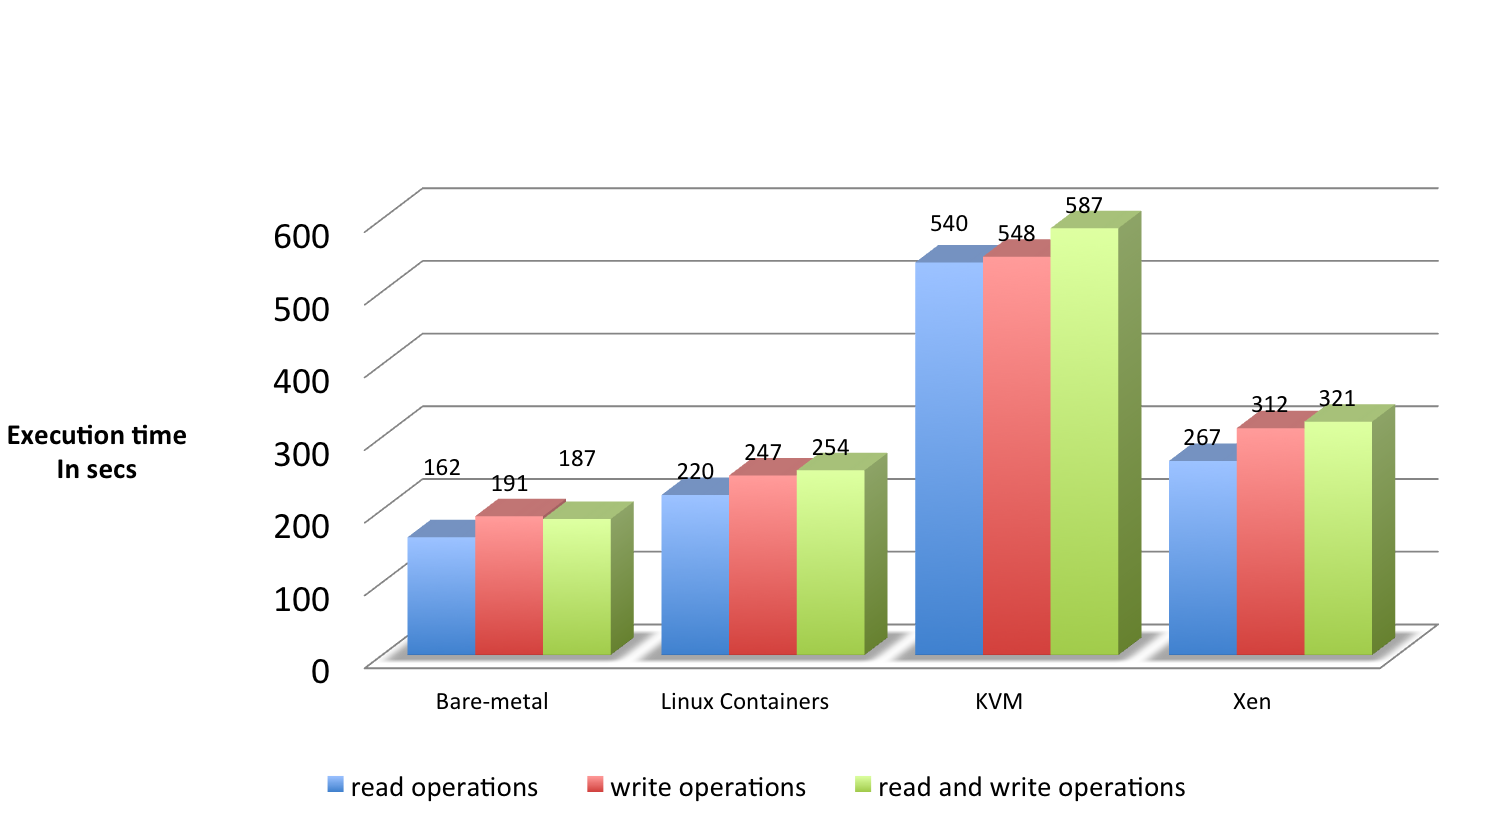
\includegraphics[width=130mm]{diskseq.png}
\caption{Virtualization Overhead - Sequential File I/O}
\label{fig:diskseq}
\end{figure}

Figure \ref{fig:diskseq} summarizes the execution time for performing 10,000 each of sequential reads, sequential writes, and mixed sequential reads and sequential writes. It is evident from the results that KVM exhibits significant overhead in virtualizing sequential I/O operations. Linux containers exhibit the least overhead, as containers do not involve any device emulation or additional drivers.

\begin{figure}[H]
\centering
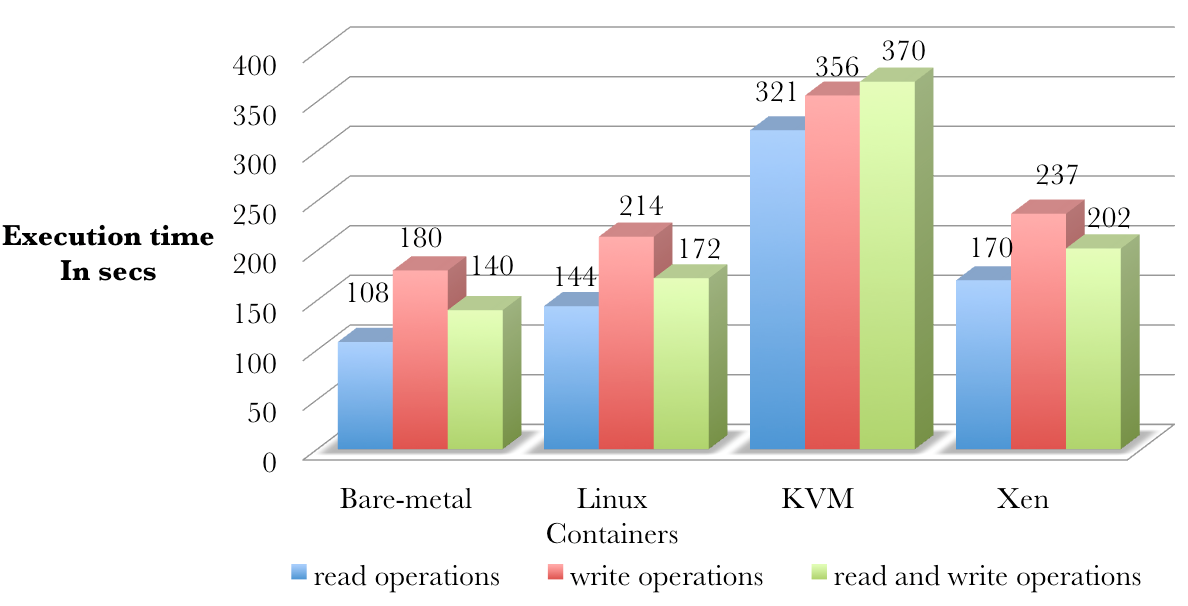
\includegraphics[width=130mm]{diskrand.png}
\caption{Virtualization Overhead - Random File I/O}
\label{fig:diskrand}
\end{figure}

Figure \ref{fig:diskrand} summarizes the execution time for performing 10,000 each of random reads, random writes, and mixed random reads and random writes. Though KVM exhibits improved performance for random I/O operations, as compared to sequential I/O operations, it is still the worst performer among the solutions. Once again, Linux Containers exhibits the least overhead in performing random I/O operations.

\begin{figure}[H]
\centering
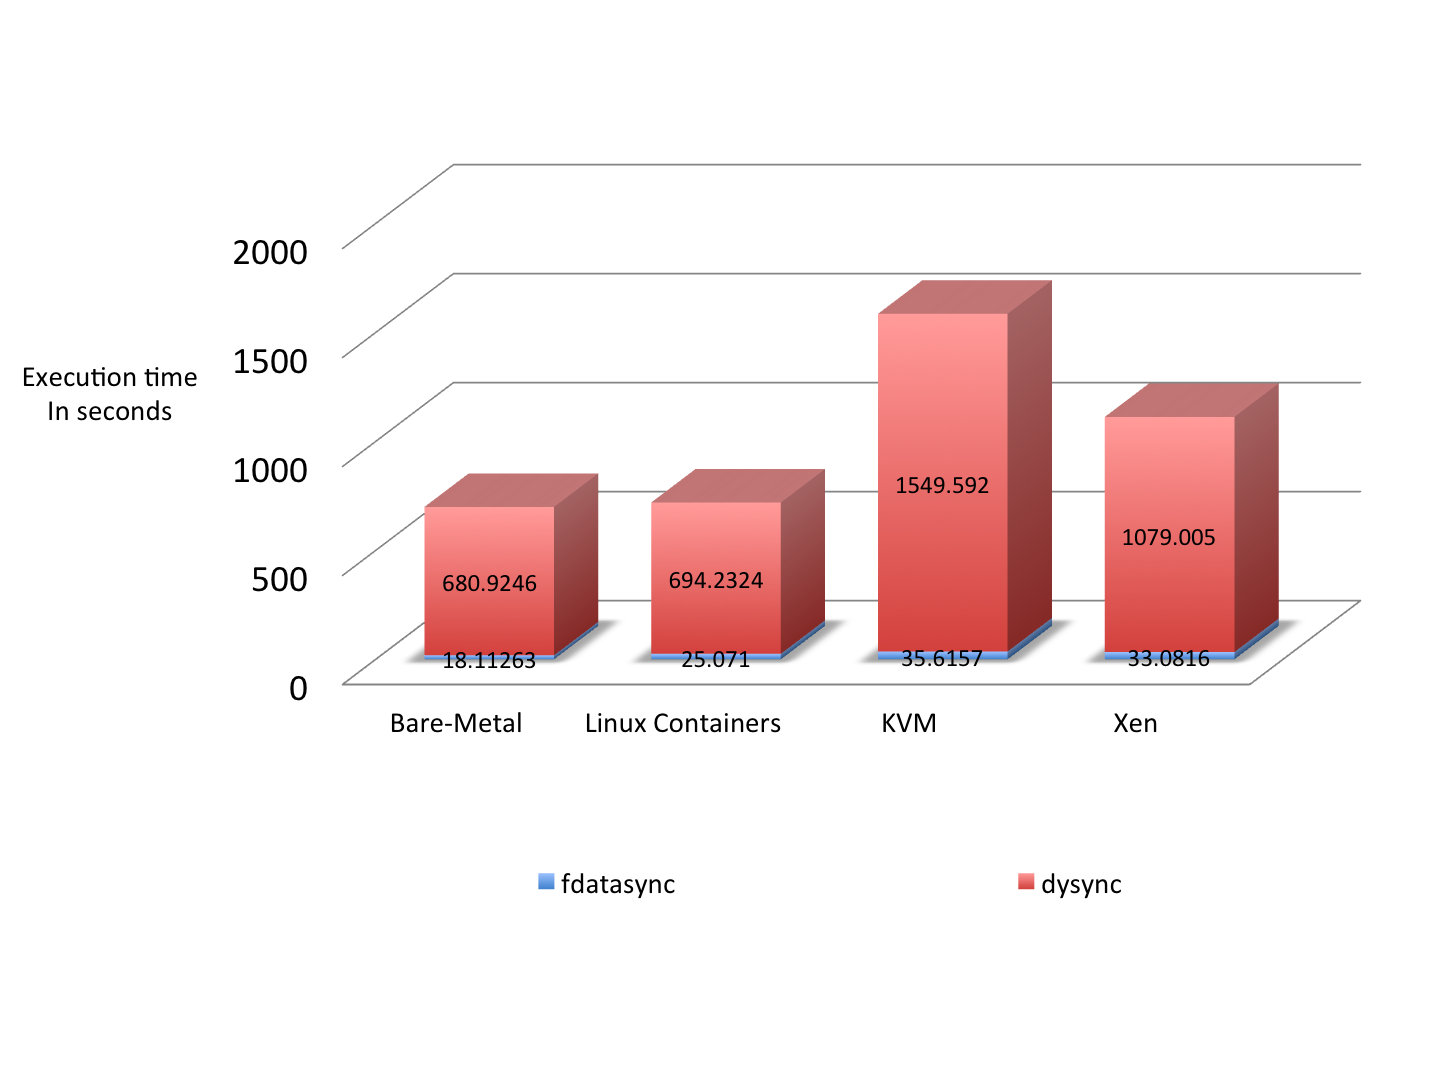
\includegraphics[width=130mm]{diskcopy.png}
\caption{Virtualization Overhead - Disk Copy Performance}
\label{fig:diskcopy}
\end{figure}

To evaluate the overhead caused by virtualization in copying files within the disk, we used the dd tool to copy a set of 1024 MB files from one location to another with the fdatasync flag (physically write output file data before finishing) and the dsync flag (use synchronized I/O for data). The results summarized in  Figure \ref{fig:diskcopy} conform to our earlier results, with KVM exhibiting the highest overhead, and Linux Containers exhibiting the least. Based on these results, we conclude that Linux Containers perform the best with respect to virtualizing disk I/O operations.   

\section{Performance Comparison - System Benchmarks}

To gauge the performance of each of the representative virtualization platforms, we analyzed the overhead they impose in order to virtualize CPU, memory, network access, and disk access. However, further evaluation based on standard system benchmarks is useful in two regards: (i) the performance of individual subsystems can be observed with little influence from other subsystems, and (ii) the results can be used to compare to prior work. This section compares the performance of each of the virtualization platforms using the LINPACK \cite{linpack}, STREAM \cite{stream}, and IOZONE \cite{iozone} benchmarks.

LINPACK is a software library that makes use of basic linear algebra subprograms to perform basic vector and matrix operations. It reflects the floating point computing performance of the CPU. The benchmark was run on a virtual machine created with 8 virtual CPUs on each of the three physical servers, and also on an independent bare-metal system used as a base-line.

\begin{figure}[H]
\centering
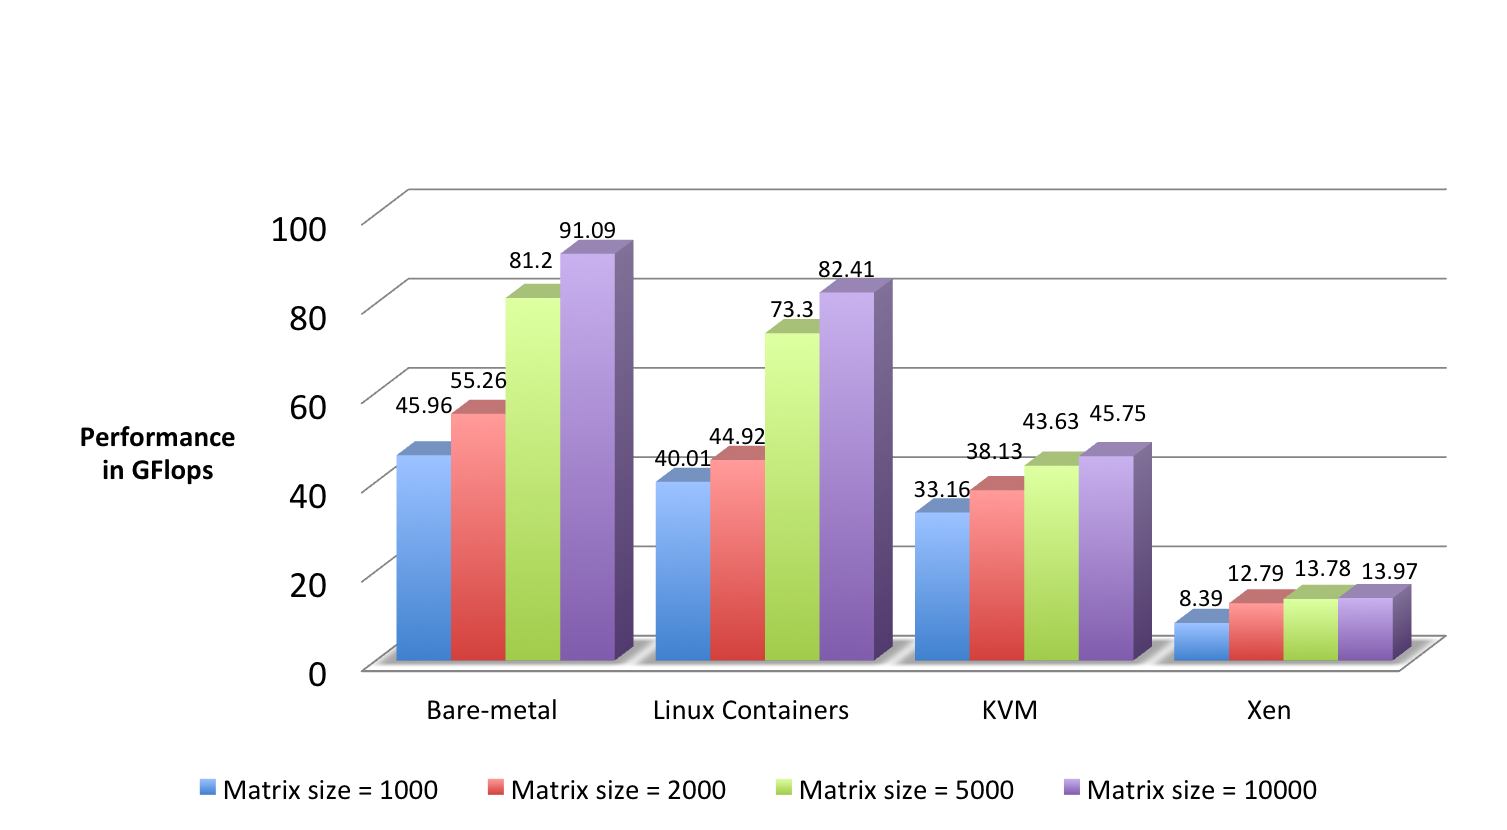
\includegraphics[width=150mm]{linpack.png}
\caption{Computing Performance using LINPACK}
\label{fig:linpack}
\end{figure}


Figure \ref{fig:linpack} summarizes the floating point performance of the virtualization platforms. The X-axis represents the virtualization platforms, and the Y-axis represents the achieved floating point performance in GFlops for different matrix sizes. It is evident from the results that Linux Containers provide near-native floating point computing performance, while Xen exhibits significantly poorer floating point computing performance. KVM performs relatively close to Linux Containers for lower matrix sizes, but the performance degrades with increased matrix sizes.

The STREAM benchmark is a simple, synthetic benchmark designed to measure sustainable memory bandwidth (in MB/s). The benchmark was run on virtual machines created with 8 virtual CPUs, and 7196 MB of memory. The benchmark was run using the ``Triad'' vector kernel.
 
\begin{figure}[H]
\centering
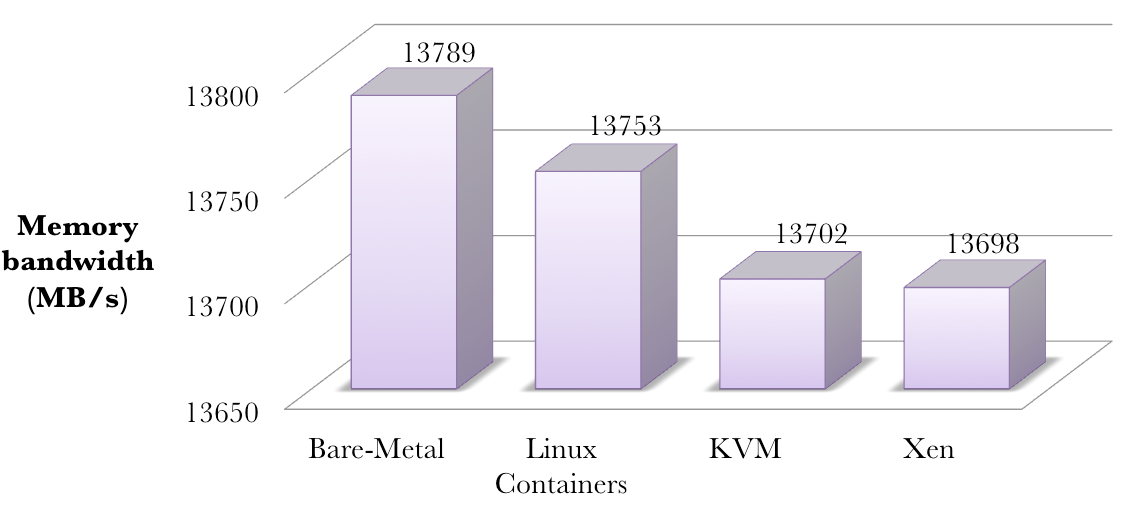
\includegraphics[width=150mm]{stream.png}
\caption{Memory Performance using STREAM}
\label{fig:stream}
\end{figure}

Figure \ref{fig:stream} summarizes the memory access performance of the virtualization platforms. The X-axis represents the virtualization platforms, and the Y-axis represents the observed memory bandwidth (in MB/s). The results corroborate our claim from the prior overhead analysis that Linux Containers provide relatively superior memory performance. KVM and Xen share similar performance. 


IOZONE is a filesystem benchmark tool that tests file I/O performance by generating a variety of file operations. The benchmark was run on virtual machines created with 8 virtual CPUs, 7196 MB of memory, and 300 GB of disk storage.

\begin{figure}[H]
        \centering
        \begin{subfigure}[b]{0.99\textwidth}
                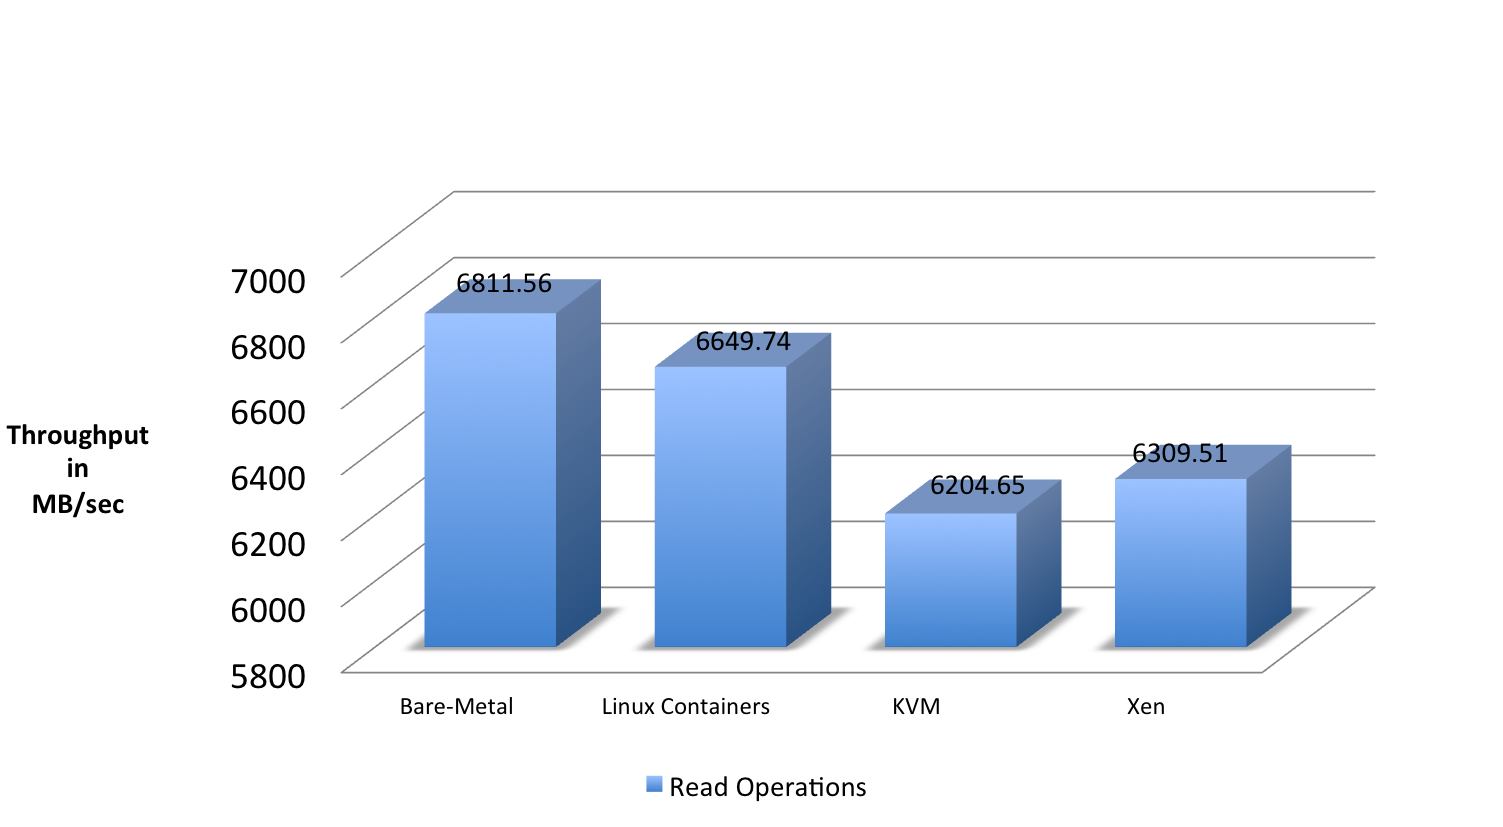
\includegraphics[width=\textwidth]{iozone_read.png}
                \caption{Read Performance}
                \label{fig:iozoneread}
        \end{subfigure}%
        \qquad \newline %\hspace{8 mm} 
        \begin{subfigure}[b]{0.8\textwidth}
                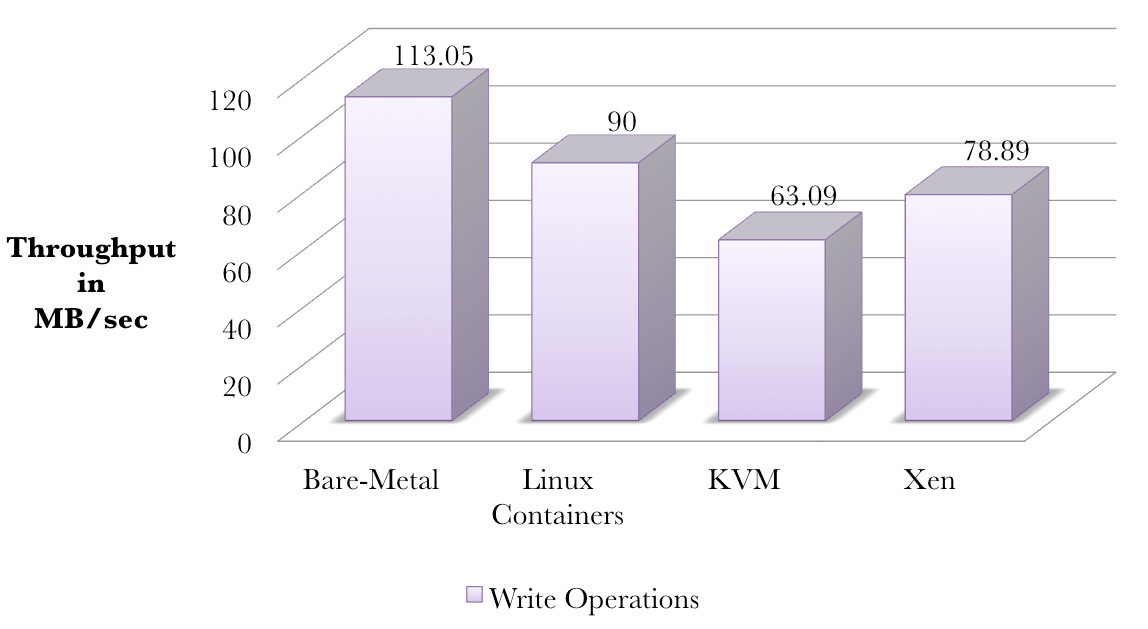
\includegraphics[width=\textwidth]{iozone_write.png}
                \caption{Write Performance}
                \label{fig:iozonewrite}
        \end{subfigure}
        \caption{Filesystem Performance using IOZONE}\label{fig:iozone}
\end{figure}

Figure \ref{fig:iozoneread} summarizes the performance of read operations on each of the virtualization platforms. The X-axis represents the virtualization platforms, and the Y-axis represents the observed read throughput (in MB/s). Linux Containers exhibited the highest read throughput, while KVM exhibited the lowest. Overall, the difference between the performance of the bare-metal host and the virtual machines does not look significant, indicating that all the platforms provide good read performance. Figure \ref{fig:iozonewrite} summarizes the performance of write operations on each of the virtualization platforms. The X-axis represents the virtualization platforms, and the Y-axis represents the observed write throughput (in MB/s). Linux Containers exhibited the highest write throughput, while KVM exhibited the lowest. 


\section{Performance Comparison - Workload-Specific Benchmarks}

This section evaluates the performance of the representative virtualization platforms with respect to specific workload categories, including web servers, database servers, and program execution environments. To identify the most suitable platform to run a web server, we tested each of the virtualization solutions using the Apache benchmark program running against an nginx web server. The benchmark was run on virtual machines created with 8 virtual CPUs, 7196 MB of memory, and 300 GB of disk storage. This test measures how many requests per second each of the systems can sustain when carrying out 500,000 requests, with upto 100 concurrent requests.

\begin{figure}[H]
\centering
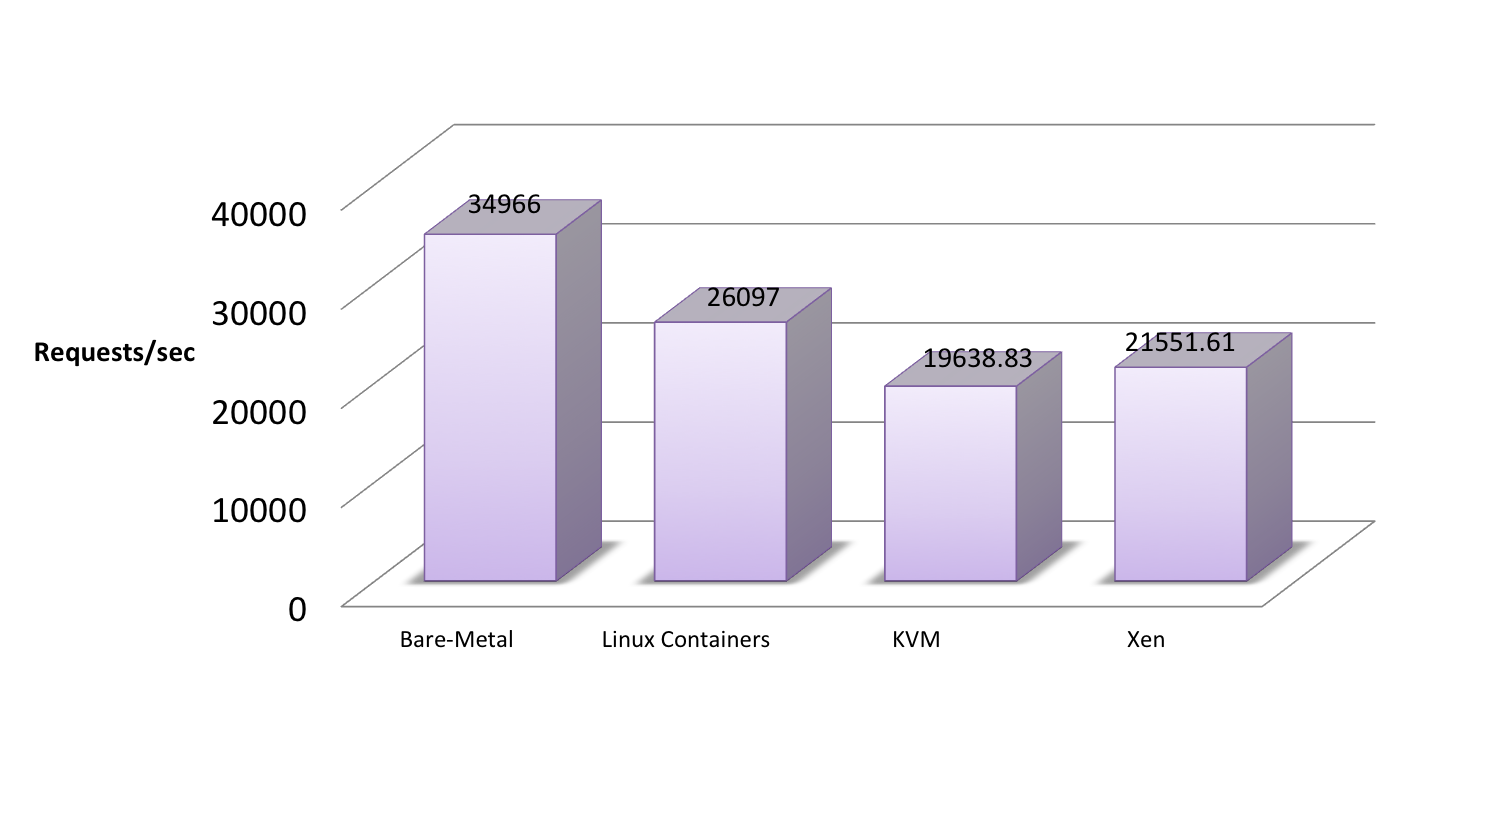
\includegraphics[width=150mm]{nginx.png}
\caption{Nginx Web Server Performance}
\label{fig:nginx}
\end{figure}

It is evident from the results summarized in Figure \ref{fig:nginx} that all of the virtualization platforms yielded low performance when compared with the bare-metal system. Linux Containers provide the highest throughput among the virtualization platforms, closely matched by Xen, while KVM yields the lowest throughput. Based on these results, Linux Containers are the preferred virtualization platform to host web servers. 


To identify the most suitable platform to run a database server, we installed PostgreSQL server on each of the virtual machines and tested the instances using the pgbench benchmark program. The benchmark was run on virtual machines created with 8 virtual CPUs, 7196 MB of memory, and 300 GB of disk storage. This test runs the same sequence of SQL commands repeatedly in multiple concurrent database sessions, and then calculates the average transaction rate (i.e., transactions per second).

\begin{figure}[H]
\centering
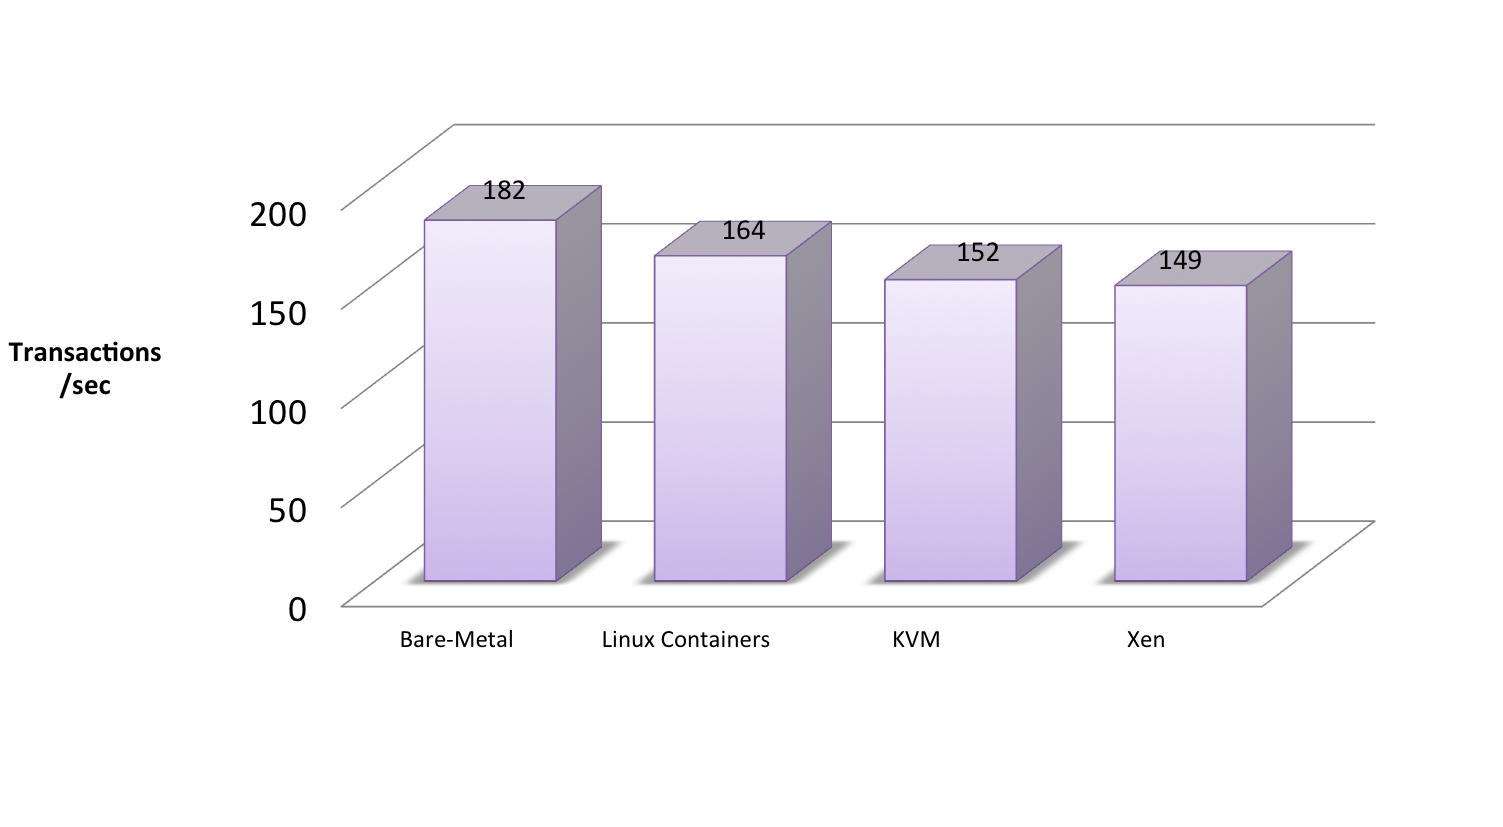
\includegraphics[width=150mm]{pgbench.png}
\caption{PostgreSQL Database Server Performance}
\label{fig:pgbench}
\end{figure}

It is evident from the results summarized in Figure \ref{fig:pgbench} that all of the virtualization platforms yielded performance very close to that provided by the bare-metal system. Linux Containers yielded the highest throughput among the virtualization platforms, closely matched by Xen and KVM. 


We chose Python and PHP to represent a custom application workload. To identify the most effective platform to run custom applications developed in Python, we setup the pybench benchmark program on virtual machines created with 8 virtual CPUs, 7196 MB of memory, and 300 GB of disk storage. This test exercises built-in functions and Python language constructs executed within nested for-loops. The result is the total execution time in seconds.

\begin{figure}[H]
\centering
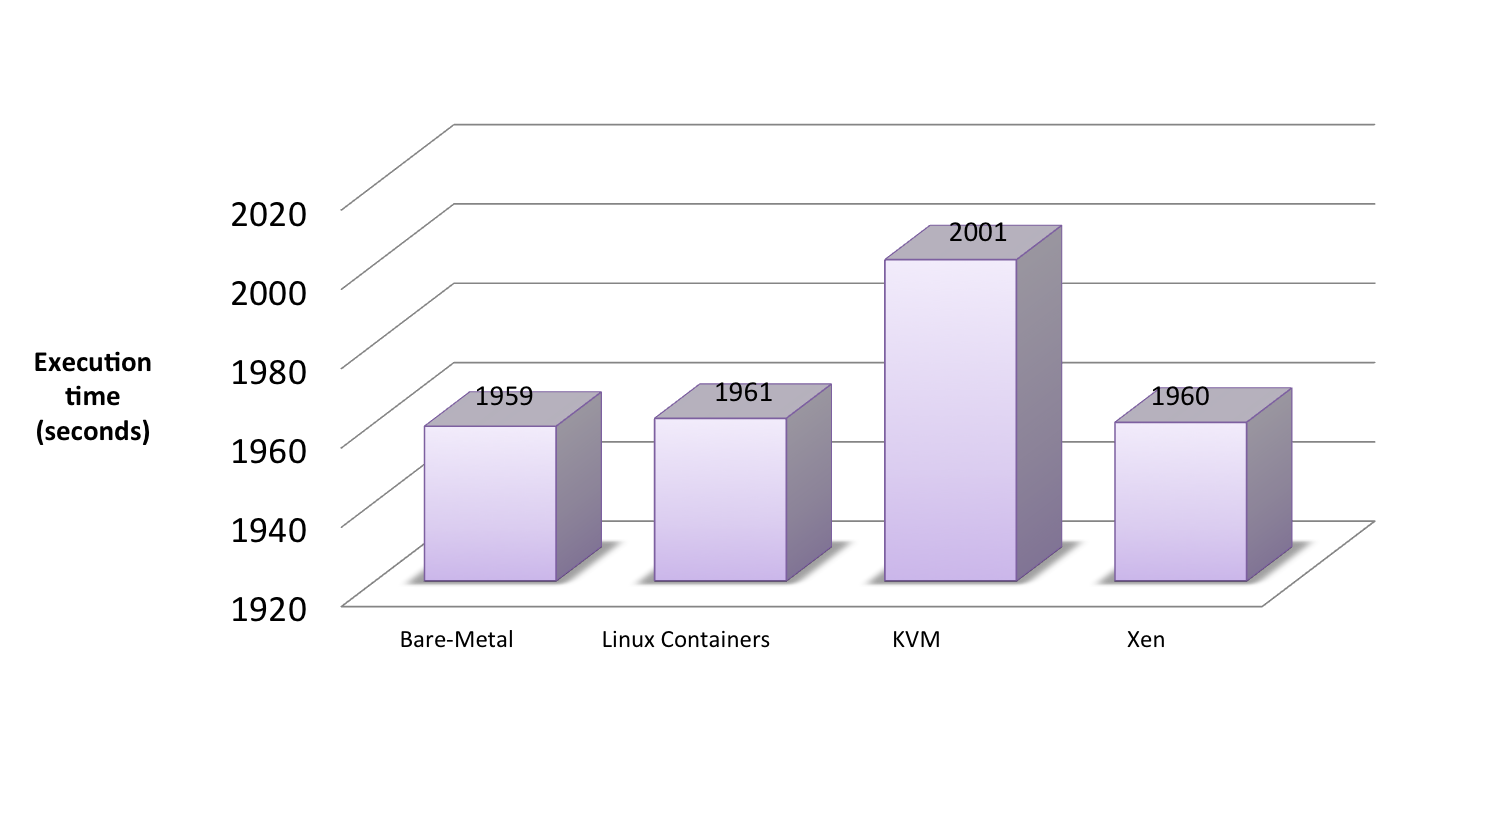
\includegraphics[width=150mm]{pybench.png}
\caption{Python Application Performance}
\label{fig:pybench}
\end{figure}

It is evident from the results summarized in Figure \ref{fig:pybench} that both Linux Containers and Xen yielded performance very close to that provided by the bare-metal system. KVM exhibited relatively low performance. 

To identify the most effective platform to run custom applications developed in PHP, we setup the phpbench benchmark program on virtual machines created with 8 virtual CPUs, 7196 MB of memory, and 300 GB of disk storage. This test exercises the PHP interpreter by executing basic PHP language constructs for 1,000,000 iterations. The result is the total execution time in seconds.

\begin{figure}[H]
\centering
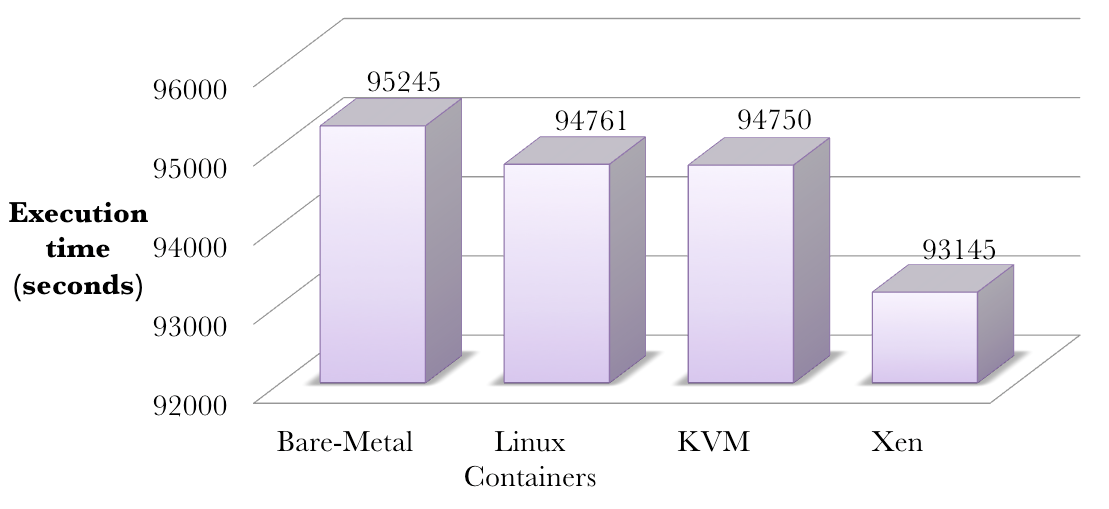
\includegraphics[width=150mm]{phpbench.png}
\caption{PHP Application Performance}
\label{fig:phpbench}
\end{figure}

It is evident from the results summarized in Figure \ref{fig:pybench} that both Linux Containers and KVM yielded performance very close to that provided by the bare-metal system. Xen exhibited relatively low performance. 

\section{Performance Comparison - Intelligent River\textsuperscript{\textregistered} Middleware}

A key motivation for this thesis is to identify the most effective virtualization platform to virtualize the Intelligent River\textsuperscript{\textregistered} middleware system. Evaluation of the virtualization platforms based on virtualization overhead, their performance on system benchmarks, and workload-specific benchmarks is not sufficient to predict each platform's performance while virtualizing a real-time middleware system. The middleware system described in Chapter 3 is a hybrid of multiple architectural patterns and is designed to scale horizontally (i.e., there can be multiple instances of every component, performing the same task in parallel). We evaluate the virtualization platforms based on the constituent middleware system components, including MongoDB, RabbitMQ, TDB, and custom observation workers.

\subsection{Virtualization Performance - MongoDB}


To evaluate the effectiveness of the platforms in virtualizing MongoDB, we created virtual machines with 8 virtual CPUs, 7196 MB of memory, and 300 GB of disk storage. We next installed MongoDB with the default configuration. We evaluate the performance of the virtual machines running MongoDB, when performing (i) insertion of documents, (ii) querying for a specific document, and (iii) updating of an existing document. To perform this evaluation, we created a test application using Java that performs these tasks. First we observe the time taken to insert 12,000 documents into a collection using 4 independent threads.


\begin{figure}[H]
\centering
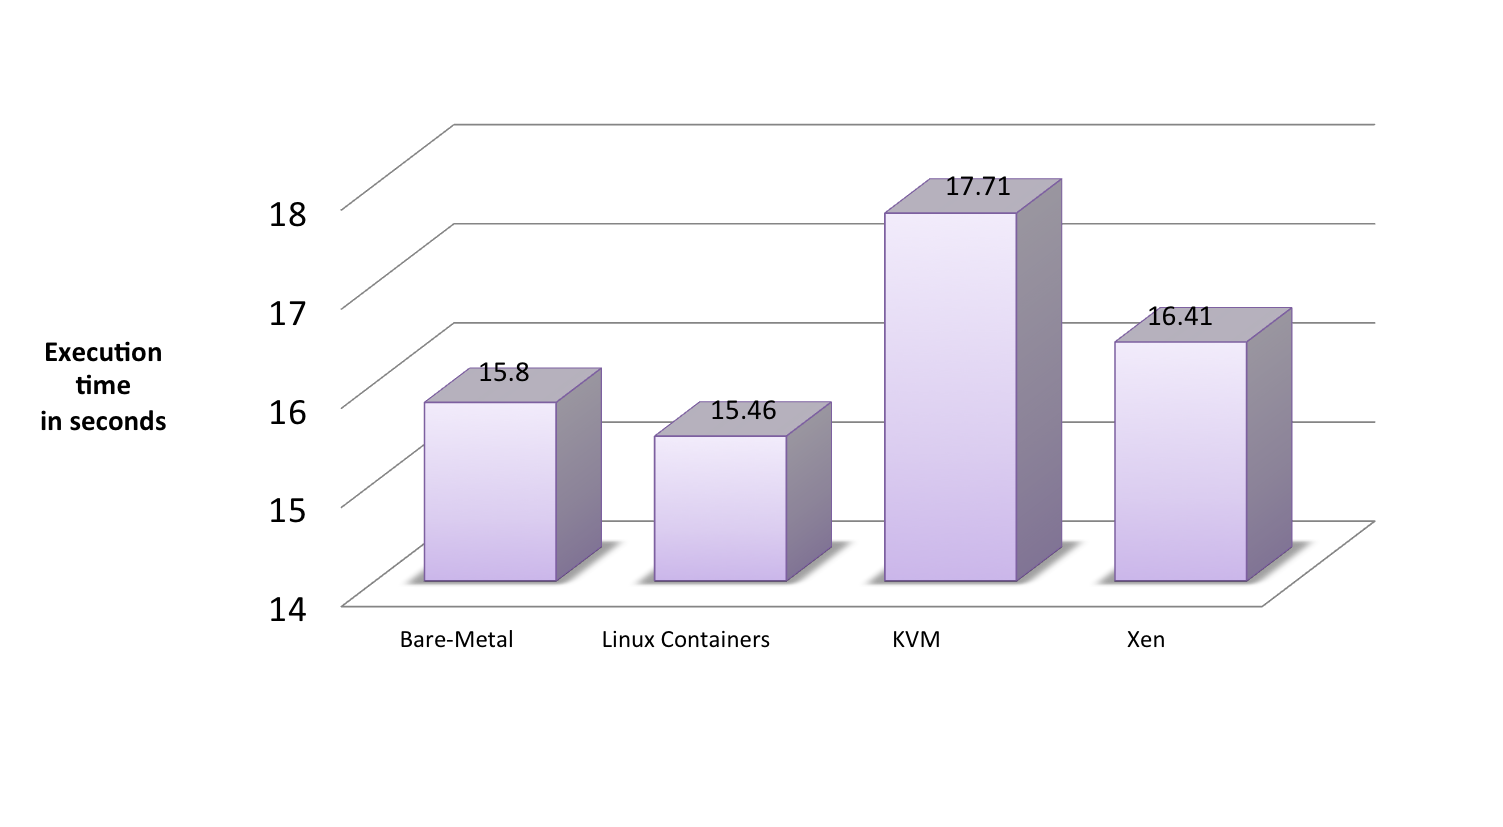
\includegraphics[width=150mm]{mongoinsert.png}
\caption{MongoDB Insert Performance}
\label{fig:mongoinsert}
\end{figure}

Interestingly, the results summarized in Figure \ref{fig:mongoinsert} show that when virtualized in a Linux container, MongoDB yielded slightly better insert throughput than the bare-metal server. The application took marginally longer to insert when virtualized with Xen compared to the bare-metal host. The KVM configuration took the longest time to complete. MongoDB operates on memory mapped files. Hence, the inserts occur in memory and are asynchronously committed to disk. We postulate that, Linux Containers yielded better performance than the bare-metal host due to the execution of fewer memory maintenance activities than the host. 

Next, we observed the time taken to execute 12,000 ``find'' queries using 4 independent threads on each of the virtualized MongoDB servers.   

\begin{figure}[H]
\centering
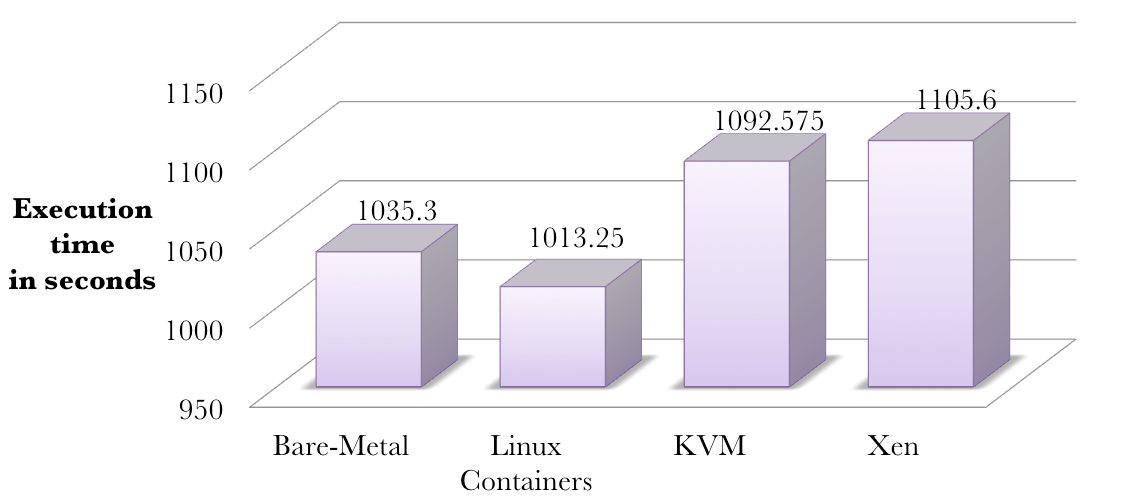
\includegraphics[width=150mm]{mongofind.png}
\caption{MongoDB Find Performance}
\label{fig:mongofind}
\end{figure}

The results summarized in Figure \ref{fig:mongofind} show that MongoDB running within a container outperforms MongoDB running on a bare-metal system when executing 12000 ``find'' queries. The MongoDB servers virtualized by KVM and Xen took significantly longer to execute the find queries. 

Finally, we observed the time taken to execute 12,000 ``set'' queries using 4 independent threads on each of the virtualized MongoDB servers.

 
\begin{figure}[H]
\centering
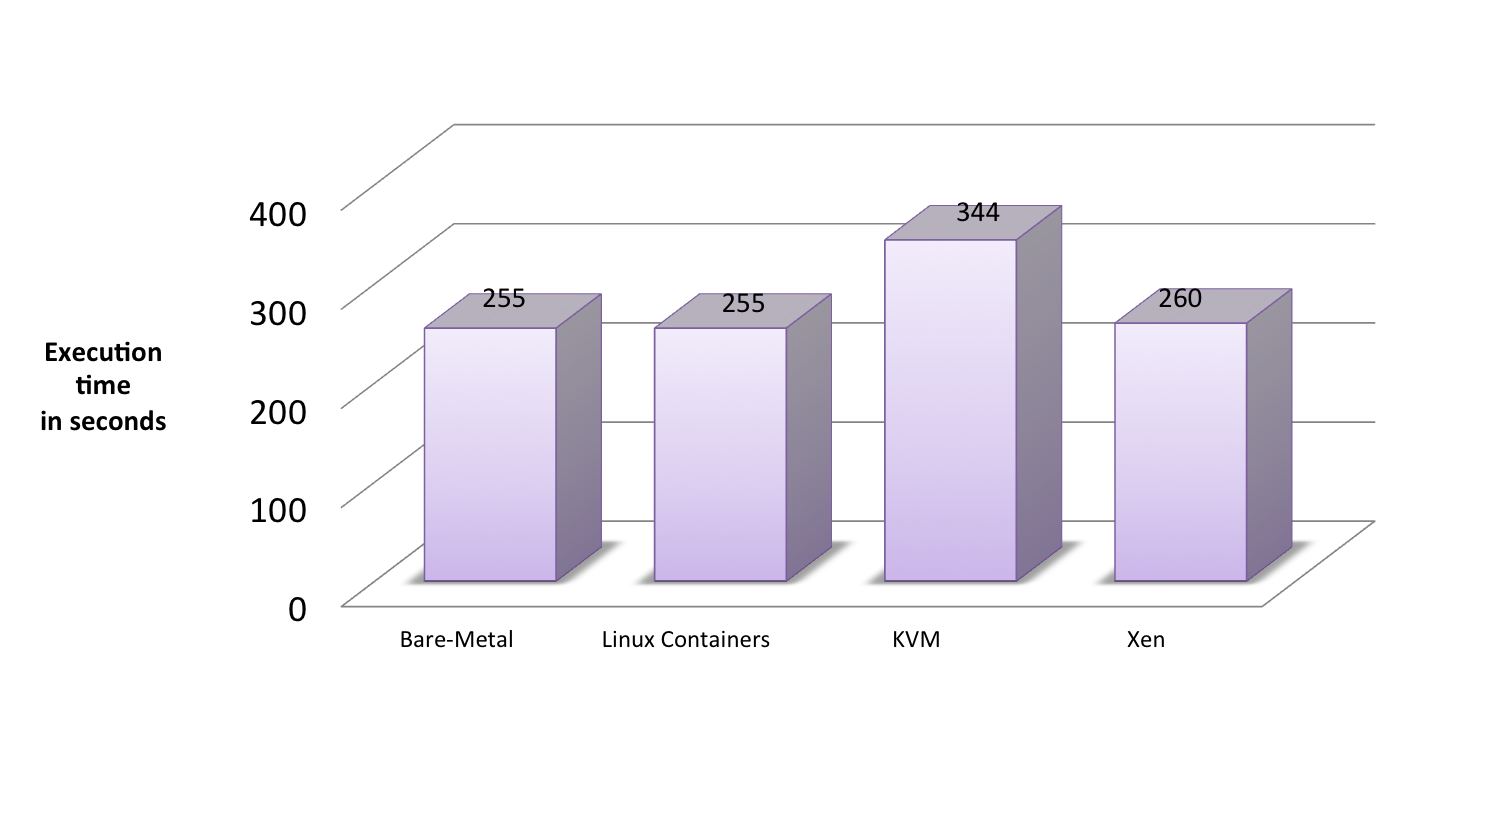
\includegraphics[width=150mm]{mongoupdate.png}
\caption{MongoDB Set Performance}
\label{fig:mongoupdate}
\end{figure}

The results summarized in Figure \ref{fig:mongofind} show that MongoDB virtualized in a container yields the same performance as MongoDB running on a bare-metal system when executing 12000 ``set'' queries. While the server virtualized with Xen yielded near-native performance, the server virtualized with KVM took significantly longer to execute the set queries. 

Based on the results presented above, Linux Containers are the preferred virtualization platform to virtualize MongoDB servers for the Intelligent River\textsuperscript{\textregistered} middleware system.

\subsection{Virtualization Performance - RabbitMQ}

RabbitMQ serves as an entry point for observations to flow into the Intelligent River\textsuperscript{\textregistered} middleware system. All middleware components communicate with each other through messages delivered via RabbitMQ. Hence, RabbitMQ is a key component of the middleware architecture. To evaluate the performance of RabbitMQ server in a virtualized environment, we observe the achieved publication throughput and the subscription throughput.

To evaluate the performance of the virtualization platforms in virtualizing RabbitMQ server, we created virtual machines with 8 virtual CPUs, 7196 MB of memory, and 300 GB of disk storage. We then installed RabbitMQ with the default configuration. To perform the evaluation, we created a Java application that publishes 50,000 observations using 8 independent threads to each of the virtualized RabbitMQ servers, and also the RabbitMQ server running on the bare-metal system.
 
\begin{figure}[H]
\centering
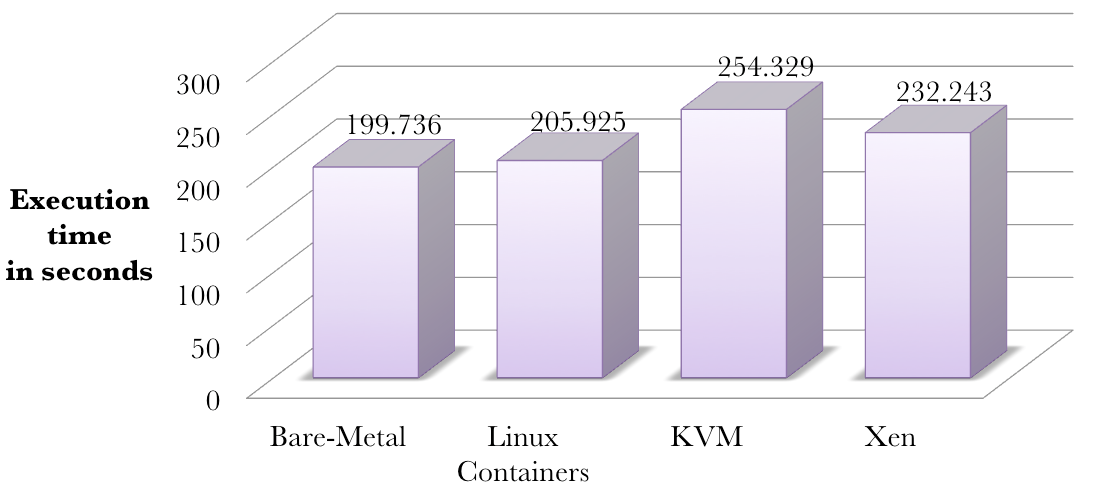
\includegraphics[width=150mm]{rabbitpub.png}
\caption{RabbitMQ Publish Performance}
\label{fig:rabbitpub}
\end{figure}

Figure \ref{fig:rabbitpub} summarizes the time taken by the application to publish 50,000 observations to RabbitMQ. It is evident from the results that Linux Containers provide near native performance, while Xen and KVM exhibit a significant decrease in the publication throughput.

Finally, to evaluate the subscription throughput of the virtualized RabbitMQ servers, we created another Java application to consume the 50,000 messages inserted during the prior evaluation. The Java application uses 8 independent threads to consume the messages.

\begin{figure}[H]
\centering
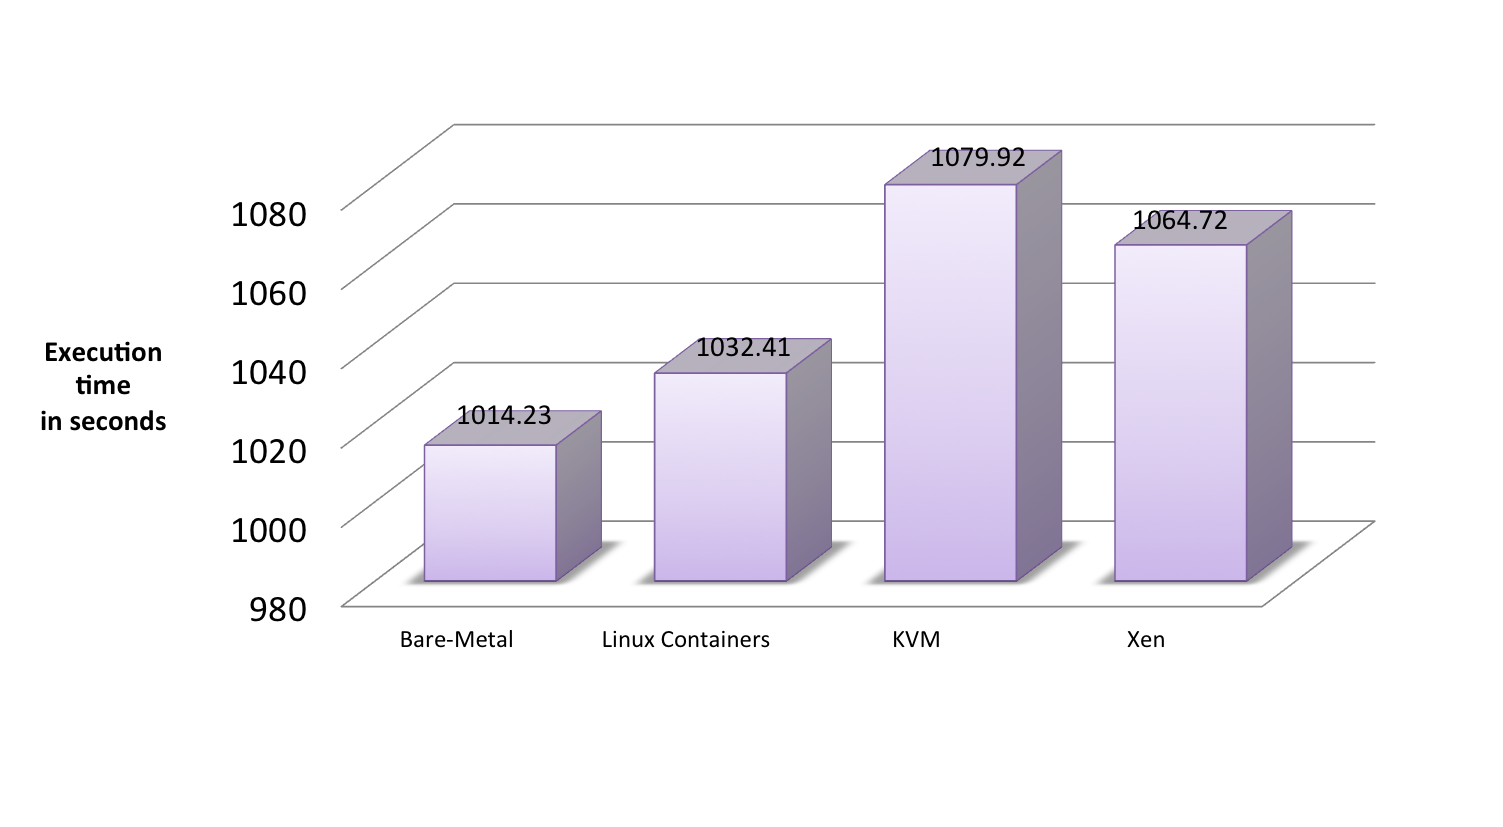
\includegraphics[width=150mm]{rabbitsub.png}
\caption{RabbitMQ Subscription Performance}
\label{fig:rabbitsub}
\end{figure}

Figure \ref{fig:rabbitsub} summarizes the time taken by the application to consume the 50,000 observations. The results once again show that Linux Containers provide near native performance, while Xen and KVM exhibit a significant decrease in the subscription throughput.

Based on the results presented above, we conclude that Linux Containers are the preferred platform to virtualize RabbitMQ servers for the Intelligent River\textsuperscript{\textregistered} middleware system.


\subsection{Virtualization Performance - Triplestore}

A triplestore is used by the middleware system to store the semantically processed observations. The two major communication patterns used to interact with the triplestore are: (i) REST API, to store and retrieve data, and (ii) SPARQL, to retrieve and process the semantic data. Since the performance of the SPARQL queries varies based on the complexity of the queries and data, we restrict the scope of this evaluation to the insertion and retrieval of semantic data through the REST API. The triplestore used by the Intelligent River\textsuperscript{\textregistered} middleware system is Apache Jena TDB. TDB stores and manages data as regular files. To evaluate the performance of TDB when virtualized using the three virtualization platforms, we created virtual machines with 8 virtual CPUs, 7196 MB of memory, and 300 GB of disk storage. We then installed TDB with the default configuration. To perform the evaluation, we created a Python script that inserts 1,000 observations.

\begin{figure}[H]
\centering
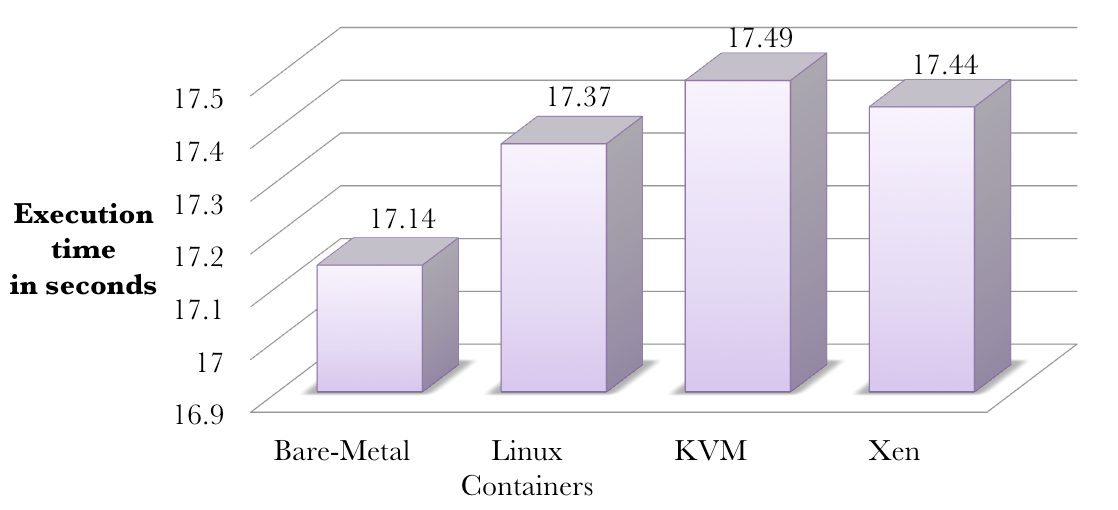
\includegraphics[width=150mm]{3storeins.png}
\caption{Triplestore Performance - Storing Observations}
\label{fig:3storeins}
\end{figure}

Figure \ref{fig:3storeins} summarizes the time taken by the script to insert 1,000 observations into TDB. It is evident from the results that all three virtualization platforms provide near native performance. 

Finally, to evaluate the retrieval performance of the virtualized TDB servers, we created another Python script that retrieves the 1,000 observations inserted during the prior test. 

\begin{figure}[H]
\centering
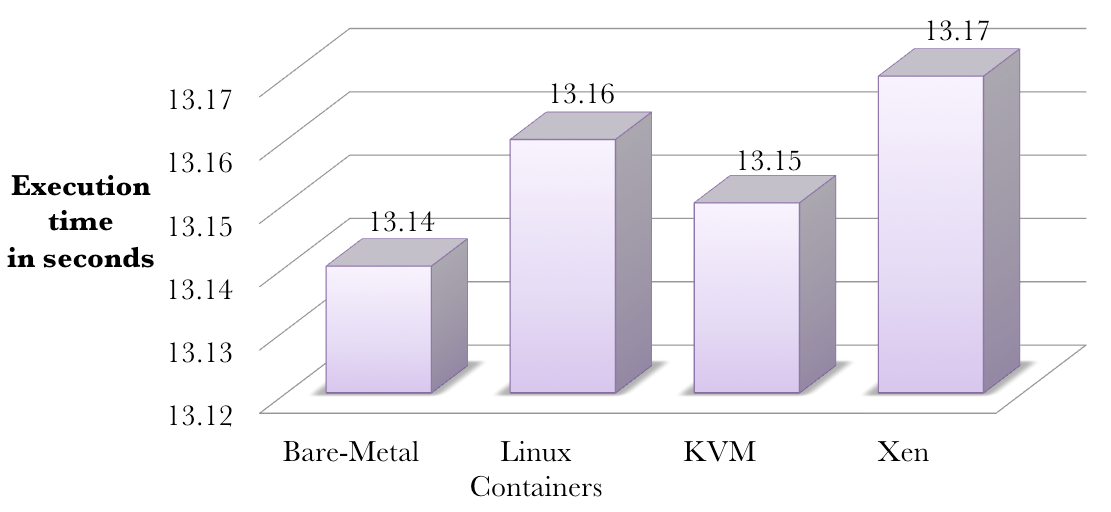
\includegraphics[width=150mm]{3storeret.png}
\caption{Triplestore Performance - Retrieving Observations}
\label{fig:3storeret}
\end{figure}

Figure \ref{fig:3storeret} summarizes the time taken to retrieve the observations. The results once again show that virtualization does not impact the performance of the TDB server.

Based on the results above, we conclude that the triplestore is not impacted by virtualization for batch insertions and retrievals.


\subsection{Virtualization Performance - Observation Workers}

Observation workers are the core components of the Intelligent River\textsuperscript{\textregistered} middleware system. The performance of an observation worker instance is dependent on the performance of all the other components of the middleware system. An instance of the observation worker application fetches the observations from RabbitMQ, inserts the observations into MongoDB, converts the observations into a semantically annotated format, and then inserts the results into the triplestore. The throughput of the observation worker can be correlated to the throughput of the entire middleware system. To evaluate its performance, we simulated an operational scenario by publishing 1,000 test observations to the RabbitMQ servers, and let the observation worker perform its processes. We observed the time taken by one instance of the observation worker to complete the processing of the 1,000 observations.


\begin{figure}[H]
\centering
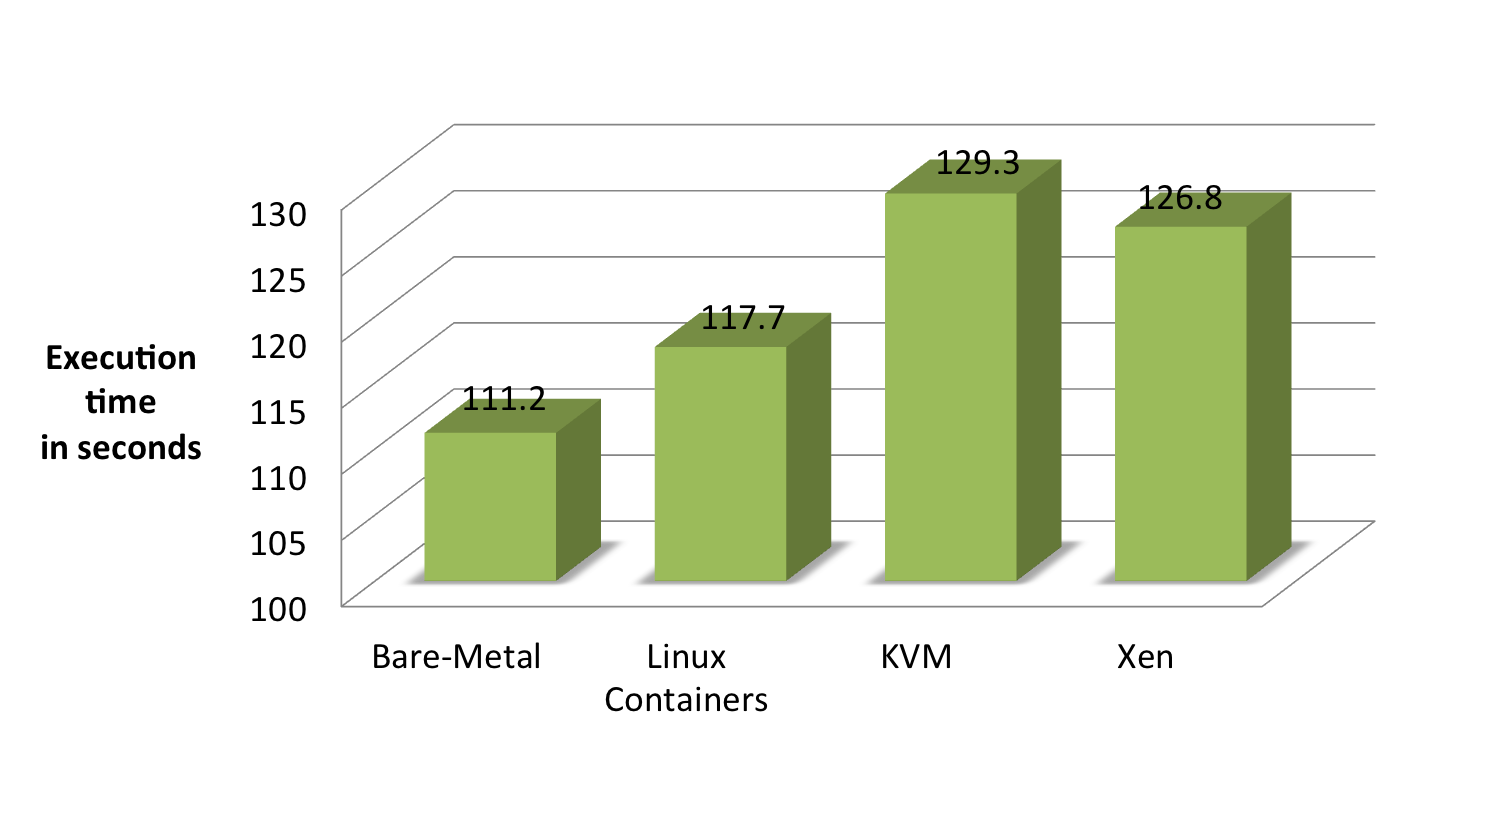
\includegraphics[width=150mm]{obsw.png}
\caption{Observation Worker Performance }
\label{fig:obsw}
\end{figure}

Figure \ref{fig:obsw} summarizes the time taken by an observation worker to complete the processing of the 1,000 observations. It is evident from the results that Linux Containers provide the best performance among the virtualization platforms in virtualizing the observation worker application.

Based on the results above, we conclude that Linux Containers are the best platform choice to virtualize the Intelligent River\textsuperscript{\textregistered} middleware system.
